\documentclass[11pt]{article}
\usepackage[margin=1in,letterpaper]{geometry}
\usepackage{amsmath,amssymb,booktabs,array,xcolor}
\usepackage[hidelinks]{hyperref}
\usepackage{graphicx}
\usepackage{tabularx}
\usepackage{caption}
\captionsetup{font=small,labelfont=bf,skip=4pt}
\usepackage{placeins}
\usepackage{tikz}
\usetikzlibrary{arrows.meta,calc}
\graphicspath{{paper_figures/}{./}{../paper_figures/}}
% More permissive float placement to reduce stranded whitespace below
% tables/figures that would otherwise defer to the next page under LaTeX's
% conservative defaults (topfraction=0.7/textfraction=0.2/etc.).
\renewcommand{\topfraction}{0.9}
\renewcommand{\bottomfraction}{0.85}
\renewcommand{\textfraction}{0.07}
\renewcommand{\floatpagefraction}{0.75}
\setcounter{topnumber}{4}
\setcounter{bottomnumber}{4}
\setcounter{totalnumber}{8}
\emergencystretch=2.5em
% Kept for a last-minute DOI fill-in if a visible marker is wanted.
% Currently unused: Data and code availability states the Zenodo/GitHub
% release will be minted at submission, with no red TODO in the PDF.
\newcommand{\todo}[1]{\par{\small\bfseries\color{red!70!black}[TODO: #1]}\par}

\title{\bfseries Exact Wave-Function Solution and Spurious-Mode Discrimination
for Completely Free Annular Sector Plates}
\author{Garrek McCune$^{a,*}$, Daniel Stutts$^{a}$\\
\small\itshape $^a$Mechanical and Aerospace Engineering,\\
Missouri University of Science and Technology, Rolla, MO 65409, USA\\
\small\upshape $^*$Corresponding author. E-mail: ghmkfh@umsystem.edu}
\date{DRAFT --- \today}
% Supplementary Material mapping (PAPER1_FREEFREE_SUPPLEMENTARY.tex):
%   S.1  former App. A (sec:frobenius-appendix)
%   S.2  former main-text appendix (B.1, Green) + (n,s) algebra
%        + closed-contour corner jump (moved from §3.3)
%        (B.3 / B.3$' already lived here)
%   S.3  former App. C minus tab:shi (now in §6.2)
%   S.3.1 / S.3.2 / S.3.3 = conv / instruments / cutoff
%   S.3.4 / S.3.5 = extensional close-pairs / Shi OOP isolation
%   S.3.6 = raw-to-physical conversion constants (moved from §6.12)
%   S.3.7 = SUBDOM numerical procedure and gate detail
%   Tables S.1--S.8 sit in S.3 (S.8 = flexural spurious zeros, was Table 7)
%   S.4  cluster job-number provenance (added 2026-08-25, advisor pass:
%        every main-text footnote job number moved here)
%   No remaining main-text appendix.

\begin{document}
\maketitle

\begin{abstract}
The Seok--Tiersten wave-function boundary-determinant method is extended
from the cantilevered annular sector to the completely free (FFFF)
configuration, in both out-of-plane (flexural) and in-plane (extensional)
motion. Frobenius-series wave functions satisfy the radial-edge conditions
exactly; a two-edge variational functional enforces the circumferential
conditions and decouples into even and odd parity blocks. Releasing both
circumferential edges leaves them enforced only weakly, which admits
spurious determinant zeros alongside the natural frequencies, so
discriminating the two becomes the central problem of the extension. The
two motion types reach different states of completeness: flexure gets a
portable, two-sided residual screen that decides a candidate from its
boundary residuals alone, on a cut calibrated once and unchanged since,
while extension's pointwise residual is one-sided on its own. Two further
extensional instruments close that gap: a portable mode-shape bar that
still requires finite-element eigenvectors, and a second, FE-free
criterion, an angle between the determinant's null direction and its own
traction-minimizing direction, that certifies a root from the boundary
determinant alone and is cluster-confirmed at four geometries and on a
full blind adjudication set of 122 candidates (70 of 77 FE modes resolved
blind, 73 once three nearest-frequency pairing defects the criterion itself
flagged in advance are corrected against independent finite-element
eigenvectors; zero duplicate zeros ever accepted). With the \S5 instruments, the
flexural tables agree with finite elements to
0.64\% (isotropic) / 1.08\% (orthotropic), with an independent literature
recovery of 6 of 6 targets at a third geometry. The extensional tables
list 26 solver roots covering
27 FE modes (one root serves the 1114.9/1115.3~Hz pair; worst
unique-partner error 0.052\%) and agree with two published
semi-analytical solutions. A two-sided
extensional bar on identity-weighted mode-shape correlation (threshold
$0.744$) classifies REAL-like versus ARTIFACT-like candidates at three
$\nu=0.30$ geometries and at all 24 extensional keys of a $\nu=0.35$
sweep; at $2\Theta/\pi=1.25$ and $1.50$ every tight FE-frequency match is
ARTIFACT-like. Two limits are reported with the rest: the tabulated
frequencies are not a certified single-pass product, since a fully-default
detector misses 4 of 26 in-plane modes, later recovered as genuine roots of
the same determinant; and one flexural FE target at
$\Omega_{\mathrm{lit}}=111.46$ remains an open assignment.
\end{abstract}

\noindent\textbf{Keywords:} annular sector plate; free vibration; exact
solution; free boundary; in-plane vibration; spurious modes;
discrimination instruments; modal assurance criterion.

\section{Introduction}
Annular and sector-shaped plates recur as vibrating components wherever a
full disk is unavailable or unconstrained: turbine and compressor
blade-disk sectors, brake and clutch friction elements, disk-type
resonators, and gear or bearing-retainer segments. The completely free
(FFFF) boundary condition treated here is the natural idealization for
such a component tested, or operating, without an external mount.
Exact solutions provide a reference standard in structural vibration
analysis that approximate methods cannot generate.
General-purpose global-basis techniques dominate engineering practice, but
their error is bounded only empirically, against a finite-element mesh
whose own convergence is itself asymptotic. An exact solution instead
supplies a reference frequency whose error is set by the retained
circumferential basis and the working precision, not by a spatial mesh,
giving approximate methods something to check their
convergence and completeness against. That role matters most where
approximate bases are weakest: dense, near-degenerate spectral regions,
such as the in-plane spectrum of a sector plate, where basis truncation
and mesh refinement both struggle to resolve closely spaced modes with
confidence.

The exact-wave-function method of Seok, Tiersten, and (for the rectangular
geometry) Scarton \cite{seok1,seok2,seok3,seok4} is one such reference
solution for annular sector and rectangular plates: the radial (or axial)
dependence is carried by
exact wave functions rather than a truncated basis, the circumferential
edge conditions are enforced through a variational functional, and natural
frequencies emerge as the zeros of a finite characteristic determinant. The
method is exact in the direction it treats analytically and spectrally
convergent in the finite direction, and the 2004 papers validated it
against contemporary numerical benchmarks to good agreement. It stopped,
however, at a single boundary configuration, the clamped-free
(cantilever) sector, and its numerical machinery (dispersion-root
tracking, branch selection, determinant assembly) was never released,
leaving the method effectively unusable by anyone outside the original
derivation.

The fully free (FFFF) sector is, among the classical boundary conditions,
the hardest one to extend the method to. The reason is structural: a
clamped edge imposes kinematic
(essential) constraints that the assumed solution can be built to satisfy
exactly, leaving only a natural (weak) condition at the opposite, free
edge; the cantilever's single free edge is accordingly the method's easiest
case. Releasing both circumferential edges removes every kinematic
constraint from the circumferential direction: both edges' conditions
become natural, enforced only in the finite Galerkin sense that the
retained wave-function basis allows, and the configuration additionally
admits rigid-body modes at zero frequency. Weak enforcement on both sides
at once admits spurious determinant zeros (nearly
displacement-free evanescent combinations that satisfy the finite
projection without satisfying the physical boundary conditions pointwise),
a failure mode with no counterpart in the cantilever case: the
clamped edge's exact kinematic satisfaction leaves no room for it to arise there.
Discriminating these spurious zeros from genuine modes is therefore the
central problem the FFFF extension must solve; the
instruments developed in \S5 address it directly.

This paper (i) documents an arbitrary-precision reimplementation, to be
released as open source alongside this paper, that reproduces the
published cantilever tables from scratch; (ii) derives and validates the extension of the boundary
determinant to two free circumferential edges, including the
edge-orientation bookkeeping this requires; (iii) identifies the resulting
spurious-zero problem and develops a pointwise edge-residual screen that
is robust and calibrated for flexural motion and is only a one-sided,
calibrated-adjudication instrument for extensional motion, together with a
basis-enlargement direction rule, an unconstrained fine-scan
arbitration step, and a two-sided extensional bar on identity-weighted
mode-shape correlation for use when FE eigenvectors are available;
(iv) reports FFFF mode tables obtained with those
instruments (not a certified single-pass detector) FE-checked in
flexure under a portable residual screen, FE-checked in extension under
a one-sided, geometry-specific residual screen, and independently
checked in extension against two published semi-analytical solutions by
direct singularity-depth agreement, with the mode-shape bar applied as a
separate instrument; (v) shows that every REAL-like flexural candidate
has its own independent finite-element partner at three further
geometries, together with a coarser 24-geometry nearest-neighbor sweep run for both motion types;
and (vi) introduces a second, FE-free extensional certification
criterion (SUBDOM) that decides a candidate from the boundary
determinant alone.

\section{Related work}
The contemporary sector-plate vibration literature is dominated by
general-boundary-condition frameworks built on approximate global bases.
Modified Fourier--Ritz formulations with supplementary edge functions,
combined with the Ritz procedure, underpin unified
first-order-shear-deformation solutions for functionally graded
\cite{wangfgm2016} and laminated composite \cite{wang2016} circular,
annular, and sector plates, and benchmark tables for graded sandwich
sector plates on two-parameter elastic foundations \cite{li2017fgm}. For
in-plane (extensional) motion specifically, the less-studied problem and
the one in which basis truncation is hardest to detect because modes
cluster densely, recent frameworks include isogeometric analysis with
NURBS bases \cite{qin2018} (its own isotropic free-free table is matched directly in \S\ref{sec:qin} below, with no FE model standing between the two), a
generalized Fourier series treatment of
annular plates with arbitrary spring-modeled edge restraints \cite{shi2014},
a modified Fourier--Ritz solution for orthotropic circular, annular, and
sector plates under general boundary conditions \cite{wangip2016} (its own
published in-plane orthotropic free-free table is checked the same way, directly, in \S\ref{sec:wang} below), and a
semi-analytical variational/multi-segment method with Jacobi-polynomial
expansions and penalty-enforced elastic constraints for composite laminated
sector and annular plates \cite{guan}. These methods owe their popularity to
flexibility: arbitrary classical or elastic edge conditions are handled by
one formulation, and convergence is demonstrated empirically against finite
elements or against each other.

This body of work has no exact counterpart (\S1): reference data come
almost exclusively from finite-element models, and the in-plane
spectrum's dense clusters and near-degenerate pairs are precisely where
that is least trustworthy. The exact-wave-function line of Seok and
Tiersten \cite{seok1,seok2,seok3,seok4} can supply that counterpart, but it
stopped in 2004 at the cantilever configuration. Independent benchmark
results exist for particular free configurations, notably the
orthotropic annular free-free material properties of Shi, Liang, Wang and Teng
\cite{shi2016}, used as the basis for an independently-run finite-element
benchmark here (\S6.2), Wang, Shi, Liang and Ahad's own published
in-plane orthotropic free-free table \cite{wangip2016}, again matched directly (\S\ref{sec:wang}), and Shi, Shi,
Li, Wang and Han's isotropic flexural free-free frequencies for annular
sector plates \cite{shi2014sector}, matched directly in
\S\ref{sec:shi2014oop}; but no systematic exact framework spans general
boundary conditions.

A separate body of work speaks directly to the difficulty this extension
runs into. Eigen-formulations that impose their boundary conditions through
a projected boundary operator rather than pointwise are known to return
spurious eigenvalues alongside the true ones, and the mechanism Chen, Lee,
Chen and Kuo \cite{chen2013} give for it is the one at work here: when part
of the constraint is dropped, the admissible solution space grows, and the
characteristic determinant acquires zeros that no physical mode
corresponds to. Lee and Chen \cite{leechen2008} analyze this for the free
vibration of circular plates under a real-part boundary integral equation
method, where discarding the imaginary-part kernel halves the computation
at the cost of spurious roots, and filter them out by adjoining constraint
equations at exterior collocating points; Ref.~\cite{chen2013} treats
annular and confocal elliptical membranes by dual BEM and the null-field
BIEM, separating the two populations through a singular value
decomposition of the discrete system and showing that true eigenvalues
depend on the boundary condition while spurious ones depend on the
formulation. The present setting differs in method --- a Frobenius
wave-function determinant rather than a boundary integral equation, with the incompleteness sitting in the circumferential Galerkin projection instead of a real-part kernel --- but the diagnosis transfers, and so does the
shape of the remedy: the instruments of \S5 are a pointwise-residual and
mode-shape analogue of the filtering those papers apply in their own
setting.

\section{Problem statement and mathematical model}
\subsection{Geometry and governing equations}
Consider an annular sector plate of inner radius $R_i$, outer radius
$R_o$, thickness $H$, sector angle $2\Theta$, density $\rho$, Young's
modulus $E$ and Poisson ratio $\nu$ (the orthotropic generalization is
summarized in \S\ref{sec:ortho}). For time-harmonic motion at circular
frequency $\omega$, the out-of-plane displacement $w(r,\theta)$ of the
classical thin-plate model satisfies
\begin{equation}
D\,\nabla^4 w \;=\; \rho H \omega^2 w, \qquad
D=\frac{EH^3}{12(1-\nu^2)},
\label{eq:oop}
\end{equation}
and the in-plane displacements $(u_r,u_\theta)$ satisfy the plane-stress
Navier equations
\begin{equation}
\frac{E}{1-\nu^2}\Big[\nabla(\nabla\!\cdot\!\mathbf{u})
-\tfrac{1-\nu}{2}\,\nabla\times(\nabla\times\mathbf{u})\Big]
\;=\;-\rho\,\omega^{2}\mathbf{u}.
\label{eq:ip}
\end{equation}
\begin{sloppypar}
Equations (\ref{eq:oop})--(\ref{eq:ip}) correspond to Ref.~\cite{seok1}
Eq.~(10) (out-of-plane, obtained there from the moment/shear-resultant
divergence after imposing zero transverse shearing strain on Mindlin's
power-series plate hierarchy, which returns classical Kirchhoff theory
rather than a first-order shear-deformable one) and Ref.~\cite{seok2} Eqs.~(9)--(10)
(in-plane, from the stress-resultant divergence). Both papers
nondimensionalize the radius as $\bar r=\pi r/2b$, $\bar r_0=\pi
r_0/(2b)$, $r^{*}=\bar r-\bar r_0$ ($b=(R_o-R_i)/2$, $r_0=(R_o+R_i)/2$)
and the frequency as $\bar\Omega=\omega/\bar\omega$ with $\bar
\omega=(\pi/2b)\sqrt{c^{*}_{66}/\rho}$ (Ref.~\cite{seok1} Eqs.~(26)--(28);
Ref.~\cite{seok2} Eqs.~(23)--(25) use the same $\bar r$, $r^{*}$ and an
analogous $\bar\Omega$). Ref.~\cite{seok1} Eq.~(27) additionally defines the
thickness-dependent scale $\bar k$, and $\bar\Omega$ enters the out-of-plane
dimensionless equation (Ref.~\cite{seok1} Eq.~(29)) only through the product
$\bar k\bar\Omega$; that product, not $\bar\Omega$ itself, is accordingly what
Ref.~\cite{seok1}'s own Table~2 tabulates and what the present work's
out-of-plane tables report as their raw column. The in-plane problem has no
such factor and reports $\bar\Omega$ directly. Both are written $\Omega$ below
where no ambiguity arises.
The out-of-plane governing equation, after separating
$w=\bar W(\bar r)\sin(\xi\theta)e^{i\Omega\bar\omega t}$, becomes the
fourth-order ODE Ref.~\cite{seok1} Eq.~(25); the in-plane displacements
$u_r,u_\theta$ separate as $\{F(\bar r)\sin(\zeta\theta),\,G(\bar
r)\cos(\zeta\theta)\}e^{i\Omega\bar\omega t}$ (Ref.~\cite{seok2} Eqs.~(19)--(20)),
giving the coupled second-order system Ref.~\cite{seok2} Eqs.~(21)--(22).
The material constants entering both are $\bar D=2h^{3}c^{*}_{11}/3$,
$\bar\nu=c^{*}_{12}/c^{*}_{11}$, $T=(2c_{66}/c^{*}_{11})+\bar\nu$,
$R^{*}=c^{*}_{22}/c^{*}_{11}$ (Ref.~\cite{seok1} Eq.~(16)), reducing to
$T=R^{*}=1$, $\bar D=D$, $\bar\nu=\nu$ for the transversely isotropic case
used throughout the present tables.
\end{sloppypar}

\begin{table}[h]\centering\footnotesize
\renewcommand{\arraystretch}{0.92}
\caption{Nomenclature: barred and nondimensional quantities introduced in
this section (isotropic case $T=R^{*}=1$, $\bar\nu=\nu$, $\bar D=D$ unless
noted), followed by the detector and discrimination-instrument symbols
used from \S4 onward.}
\label{tab:nomenclature}
\begin{tabularx}{\linewidth}{@{}lX@{}}
\toprule Symbol & Definition\\ \midrule
$b=(R_o-R_i)/2$ & half radial width\\
$r_0=(R_o+R_i)/2$ & center (expansion) radius\\
$\bar r=\pi r/2b$ & nondimensional radius\\
$\bar r_0=\pi r_0/2b$ & nondimensional center radius\\
$r^{*}=\bar r-\bar r_0$ & shifted radial expansion variable\\
$\bar\Omega=\omega/\bar\omega$ & nondimensional frequency of Refs.~\cite{seok1,seok2}\\
$\Omega$ & raw solver frequency: $\Omega=\bar\Omega$ (in-plane),
$\Omega=\bar k\bar\Omega$ (out-of-plane); Supplementary Material, §S.3.6\\
$\bar\omega=(\pi/2b)\sqrt{c^{*}_{66}/\rho}$ & in-plane frequency scale\\
$\bar k$ & out-of-plane (thickness-dependent) wavenumber scale (Supplementary Material, §S.3.6)\\
$\Omega_{\mathrm{lit}}=\omega R_o^2\sqrt{\rho H/D}$ & classical out-of-plane literature frequency ratio\\
$\Omega_{\mathrm{Wang}},\ \Omega_{\mathrm{Qin}}$ & source-specific in-plane frequency parameters, each defined where first used (\S\ref{sec:wang}, \S\ref{sec:qin})\\
$\bar D=2h^{3}c^{*}_{11}/3$ & nondimensional flexural rigidity ($h=H/2$)\\
$\bar\nu=c^{*}_{12}/c^{*}_{11}$ & nondimensional Poisson-type ratio\\
$T=(2c_{66}/c^{*}_{11})+\bar\nu$ & dimensionless orthotropic constant\\
$R^{*}=c^{*}_{22}/c^{*}_{11}$ & dimensionless orthotropic constant\\
\addlinespace[2pt]
$\sigma_{\min}$ & smallest singular value of $\mathbf{K}(\Omega)$; ``depth'' means $\log_{10}\sigma_{\min}$ (\S4)\\
$n_{\mathrm{dofs}}$ & generalized coordinates retained in $\mathbf{K}$ (\S4)\\
$\Omega^{*}$ & a converged, bracket-stable root of $\det\mathbf{K}(\Omega)=0$\\
$r_M,\ r_V$ & flexural moment / effective-shear edge-residual ratios (\S5)\\
$r_{\theta\theta},\ r_{\theta r}$ & extensional normal- / shear-traction edge-residual ratios (\S5)\\
MAC & identity-weighted modal assurance criterion (\S\ref{sec:ipmacbar})\\
$\mathbf{D},\mathbf{T}$ & displacement- / traction-weight matrices of $\mathbf{K}=\mathbf{D}^{\mathsf T}\mathbf{T}$ (\S\ref{sec:subdom}); bold, distinct from the scalars $D$, $T$ above\\
$\eta(c),\ \eta(\Omega)$ & traction-to-displacement ratio at a coefficient vector, and its minimum over all of them (\S\ref{sec:subdom})\\
$\gamma,\ p$ & degeneracy-pooling factor ($\gamma=4$) and the resulting number of pooled lowest-traction directions (\S\ref{sec:subdom})\\
SUBDOM & interior-field subspace-dominance criterion; the call is SUBDOM~$>0.70$ (\S\ref{sec:subdom})\\
\bottomrule
\end{tabularx}
\renewcommand{\arraystretch}{1}
\end{table}

The radial edges $r=R_i,R_o$ carry the papers' exactly satisfied
conditions; the circumferential edges $\theta=\pm\Theta$ carry, in the
present work, the free conditions: vanishing bending moment and effective
(Kelvin--Kirchhoff) shear for out-of-plane motion, and vanishing normal and shear
tractions $T_{\theta\theta}=T_{\theta r}=0$ for in-plane motion.
\begin{figure}[h]\centering
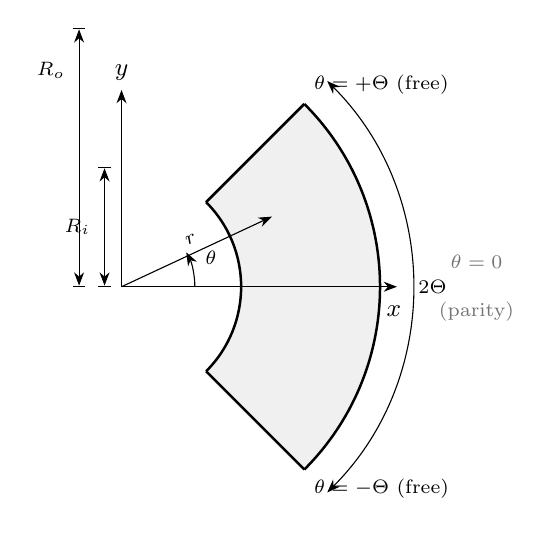
\begin{tikzpicture}[scale=0.98, >=Stealth, font=\small]
  \def\Ri{1.55}
  \def\Ro{3.35}
  \def\Th{45}
  % plate
  \fill[black!6]
    (\Th:\Ri) arc (\Th:-\Th:\Ri) -- (-\Th:\Ro) arc (-\Th:\Th:\Ro) -- cycle;
  \draw[line width=0.9pt]
    (\Th:\Ri) arc (\Th:-\Th:\Ri)
    (-\Th:\Ro) arc (-\Th:\Th:\Ro);
  \draw[line width=0.9pt] (\Th:\Ri) -- (\Th:\Ro);
  \draw[line width=0.9pt] (-\Th:\Ri) -- (-\Th:\Ro);
  % bisector / parity
  \draw[dashed, black!50] (0,0) -- (\Ro+0.12,0);
  \node[font=\scriptsize, black!55] at (\Ro+1.25,0.32) {$\theta=0$};
  \node[font=\scriptsize, black!55] at (\Ro+1.25,-0.32) {(parity)};
  % polar frame: stop the x-axis before the $2\Theta$ label
  \draw[->] (0,0) -- (\Ro+0.22,0);
  \draw[->] (0,0) -- (0,2.55) node[above] {$y$};
  \node[anchor=north] at (\Ro+0.18,-0.12) {$x$};
  \draw[->] (0,0) -- (25:2.15) node[midway, above, sloped, font=\scriptsize] {$r$};
  \draw[->] (0.95,0) arc (0:28:0.95);
  \node[font=\scriptsize] at (18:1.22) {$\theta$};
  % edge labels (Ri, Ro already marked by the left dimension arrows)
  \node[font=\scriptsize, align=center, anchor=south west] at (\Th:\Ro)
    {$\theta=+\Theta$ (free)};
  \node[font=\scriptsize, align=center, anchor=north west] at (-\Th:\Ro)
    {$\theta=-\Theta$ (free)};
  % 2 Theta arc
  \draw[<->] (\Th:\Ro+0.42) arc (\Th:-\Th:\Ro+0.42);
  \node[font=\scriptsize] at (0:\Ro+0.68) {$2\Theta$};
  % Ri, Ro ticks
  \draw[|<->|] (-0.22,0) -- (-0.22,\Ri);
  \node[font=\scriptsize, anchor=east] at (-0.28,{\Ri/2}) {$R_i$};
  \draw[|<->|] (-0.55,0) -- (-0.55,\Ro);
  \node[font=\scriptsize, anchor=east] at (-0.61,{(\Ri+\Ro)/2+0.35}) {$R_o$};
\end{tikzpicture}
\caption{Annular sector: radial edges $r=R_i,R_o$ exact; circumferential
edges $\theta=\pm\Theta$ free. Primary benchmark $2\Theta=\pi/2$;
\S\ref{sec:r150a100} also treats $2\Theta=\pi$ and $R_i/R_o=0.6$;
\S\ref{sec:geomsweep}'s sweep spans further radius ratios and sector
angles on the same schematic.}
\label{fig:geometry}
\end{figure}
The isotropic free-free tables of \S6 use a single physical plate
($R_i=4$~m, $R_o=8$~m, $H=0.08$~m, $2\Theta=\pi/2$, steel
$E=210$~GPa, $\nu=0.30$, $\rho=7800$~kg/m$^3$), for which
$\bar\omega=2527.351$~rad/s and $\bar k=32.617$: in-plane raw output is
already $\bar\Omega=\omega/\bar\omega$, out-of-plane raw output is the
product $\bar k\bar\Omega$. The conversion algebra and the eight-row
numerical cross-check against Table~\ref{tab:oop} are in Supplementary
Material, §S.3.6.

\subsection{Exact radial wave functions}
Separating $w=W(r)\,\{\sin,\cos\}(\xi\theta)$ (and correspondingly for
$u_r,u_\theta$ with transverse wavenumber $\zeta$) reduces
(\ref{eq:oop})--(\ref{eq:ip}) to ordinary differential equations in $r$
whose solutions are constructed as Frobenius series about the center
radius $r_0$. For each frequency the admissible transverse wavenumbers are the
roots of the radial-edge dispersion relation; the root set comprises
real, imaginary, and complex families, all of which must be retained. The
basis is assembled by a census-and-fill procedure that tracks every branch
across frequency; dropping a family produces silent mode loss, and branch
completeness proved to be the practically difficult part of replication.
Following Ref.~\cite{seok1} \S3 (out-of-plane) and Ref.~\cite{seok2} \S3
(in-plane), each expansion is taken about $r_0$, not the singular
point $r=0$, guaranteeing four independent solutions regular on the
plate; the recursion for the series coefficients, which the source papers
describe as ``much too cumbersome to include'' in closed form, is carried
numerically to convergence at working precision (\texttt{mpmath}, 40
digits) instead of being truncated at a fixed low order as the papers'
fixed-precision Maple calculation could tolerate. The full
indicial-equation and four-branch selection detail, and the branch-census
construction (tracking what the papers' own dispersion curves,
Ref.~\cite{seok1} Fig.~2, exhibit), are given in Supplementary
Material, §S.1.

\subsection{Two-edge variational functional and parity decomposition}
The circumferential-edge conditions are enforced through the papers'
variational functional, projected onto the retained basis of $n$ wave
functions, giving the boundary matrix $\mathbf{K}(\Omega)\in
\mathbb{R}^{n\times n}$; natural frequencies satisfy
$\det\mathbf{K}(\Omega)=0$. For the cantilever, the clamped edge
contributes kinematic rows and the free edge natural rows. For the
free-free plate both edges contribute natural rows, and the two
contributions carry opposite orientation signs; with the orientation
carried correctly the matrix decouples exactly into even and odd
angular-parity blocks,
$\mathbf{K}=\mathrm{diag}(\mathbf{K}^{e},\mathbf{K}^{o})$, halving the
computation and assigning each mode a definite parity. (If the sign is
instead dropped, the same-parity contributions cancel identically for
arbitrary radial content: a structural cancellation demonstrated
algebraically later in this subsection.)
The papers derive this functional for the single-free-edge cantilever, in
which one circumferential edge ($\theta=\Theta$) is free and the other
($\theta=-\Theta$) is clamped: once the radial-edge conditions, already
satisfied exactly by the wave functions of \S3.2, are used to
eliminate the bulk term, what remains is the corner-bearing form
Ref.~\cite{seok1} Eq.~(43) for out-of-plane motion (Ref.~\cite{seok2}
Eq.~(48) for in-plane), giving the assembled system $\mathbf{K}\mathbf{X}=0$
(Ref.~\cite{seok1} Eq.~(46)) with $\mathbf{X}$ the per-branch, per-parity
amplitude coefficients (Eq.~(47)). Eq.~(43)'s tail carries \emph{two}
corner terms, and it is essential to the free-free derivation to see that
they are not the same term at two locations: each is a jump contribution
over the two radial edges, $r^{*}=\pm\pi/2$, but evaluated at a single,
different circumferential edge apiece: coefficient $+(T-\bar\nu)$ at the
\emph{clamped} edge $\theta=-\Theta$, and coefficient $-2(T-\bar\nu)$ at the
\emph{free} edge $\theta=\Theta$ (transcribed verbatim in
Supplementary Material, §S.2, Eq.~(B.1)). The clamped-edge term arises
from the paper's Lagrange-type substitution enforcing $w=\partial
w/\partial\theta=0$ at $\theta=-\Theta$; the free-edge term is the genuine
free-edge natural boundary contribution. These are two structurally
different derivations that happen to multiply the same combination
$(T-\bar\nu)$. The same wall/tip asymmetry recurs in three source-paper
cases: the present annular Eq.~(43), the rectangular out-of-plane case
(Ref.~\cite{seok3} Eq.~(53)), and the rectangular in-plane case
(Ref.~\cite{seok4} Eq.~(36)). The
free-free plate's $\theta=-\Theta$ corner term must therefore reuse the
\emph{free}-edge formula, $-2(T-\bar\nu)$, re-evaluated at $\theta=-\Theta$
with the correct relative orientation, not Eq.~(43)'s clamped-edge
coefficient. The remainder of this subsection states the resulting free-free
corner-term formula and proves the same-parity cancellation of the
mis-oriented assembly. The closed-contour $(n,s)$ table, the four
corner jumps, and the surface-term substitution this builds on are in
Supplementary Material, §S.2.

\paragraph{The corner-jump derivation.} Ref.~\cite{seok1} Eq.~(6),
reproduced in full in Supplementary Material, §S.2 (Eq.~(B.2)), has
its own asymmetric corner factors ($-1$ at $\theta=-\Theta$, $+2$ at
$\theta=\Theta$), which reflect that, in the cantilever's contour $C_N$,
a free $\theta=\Theta$ corner is where two free edges meet, while the
$\theta=-\Theta$ corner sits where $C_N$ terminates at the wall. For the
free-free case $C_N$ becomes the full closed boundary, and the corner
coefficient follows from Eq.~(1a)'s fourth term
$\int_{c_N}\!ds\,(n_a\tau^{(1)}_{a\beta}s_\beta\,\delta w)_{,s}$:
$n_a,s_b$ are discontinuous at each corner even though the physical
stress $\tau^{(1)}_{r\theta}$ is continuous there. Writing
$F\equiv n_a\tau^{(1)}_{a\beta}s_\beta$ on each segment of that closed
contour (Supplementary Material, §S.2) and taking the jump as incoming
$F$ minus outgoing $F$ gives magnitude 2 at every corner, alternating in
sign between the two edge pairs: the $\theta=\Theta$ pair reproduces
Ref.~\cite{seok1}'s printed cantilever corner term exactly, and the
$\theta=-\Theta$ pair, now smooth-turn corners of the closed contour,
gives the free-edge coefficient $-2$ with the same orientation sign
already used for every corner, so the identical $\pm1$ orientation factor
that fixes the sign of Eq.~(B.3$'$) (Supplementary Material, §S.2) also
fixes the corner term's. Substituting
the remaining constitutive relation this term needs,
\begin{equation}
\tau^{(1)}_{r\theta}=-\bar D(T-\bar\nu)\frac{\partial^2}{\partial
r\partial\theta}\Big(\frac{w}{r}\Big),
\tag{Ref.~\cite{seok1} Eq.~(15)}
\end{equation}
and the same nondimensionalization as Supplementary Material, §S.2
turns this jump result into the free-free analogue of Eq.~(43),
\begin{equation}
+2(T-\bar\nu)\Big[\tfrac{\partial^2}{\partial r^{*}\partial\theta}
\Big\{\tfrac{w}{r^{*}+\bar r_0}\Big\}\Big]_{r^{*}=-\pi/2,\,\theta=-\Theta}^{r^{*}=\pi/2,\,\theta=-\Theta}
-2(T-\bar\nu)\Big[\tfrac{\partial^2}{\partial r^{*}\partial\theta}
\Big\{\tfrac{w}{r^{*}+\bar r_0}\Big\}\Big]_{r^{*}=-\pi/2,\,\theta=\Theta}^{r^{*}=\pi/2,\,\theta=\Theta}=0.
\label{eq:corner-jump-result}
\end{equation}
Magnitude and alternation follow from the contour argument just given
and from an independent Green's-identity argument (a bilinear-form
check on the classical constant pure-twist field, Supplementary
Material, §S.2) that reproduces the same free-edge magnitude and
factor of 2 by a code- and FE-independent route. What neither argument
assigns on its own is which isolated edge carries the ``$+$'' label --- but
that is a convention of the overall stationarity condition rather than
physical content: multiplying the whole equation by $-1$ swaps both labels
and moves no frequency. What has to be consistent is the \emph{relative}
sign between the corner term and the surface term inside the same
equation, and it is: the identical $\pm1$ orientation factor fixes both,
and the implemented assembly applies that one rule on both free edges. No
finite-element result or published value enters at this step; \S6's FE
comparison tests the completed assembly rather than supplying any
coefficient in it.

\paragraph{Orientation and the same-parity cancellation proof.} Write each
retained basis function's angular factor as $\sin(\xi\theta+q\pi/2)$,
$q\in\{0,1\}$ ($q=0$: the $\sin$, angularly ODD family; $q=1$: the $\cos$,
angularly EVEN family, since $\sin(\xi\theta+\pi/2)=\cos(\xi\theta)$).
Evaluating the identical factor at the mirror edge $\theta\to-\theta$,
\[
\sin(-\xi\theta+q\pi/2) = (-1)^{\,1-q}\,\sin(\xi\theta+q\pi/2)
\quad\Longleftrightarrow\quad
\begin{cases}
q=0: & \sin(-\xi\theta)=-\sin(\xi\theta)\ \ \text{(sign flips)},\\
q=1: & \cos(-\xi\theta)=\cos(\xi\theta)\ \ \text{(sign fixed)}.
\end{cases}
\]
A boundary-matrix entry $K_{ij}$ pairs a test function $i$ and a trial
function $j$, each carrying its own parity label $q_i,q_j\in\{0,1\}$, and
the free-edge pairing mixes a stress factor of one with a displacement
factor of the other.
Writing $\sigma(q)=-1$ for $q=0$ and $+1$ for $q=1$, the free-edge pairing
is a mixed $\sin$/$\cos$ projection (one function's stress factor times the
other's displacement factor), so it is odd in the edge sign for SAME-parity
pairs. The unsigned functional evaluated at $\theta=-\Theta$ therefore equals
$-\sigma(q_i)\sigma(q_j)$ times its value at $\theta=\Theta$: $-1$ whenever
$q_i=q_j$ (SAME parity) and $+1$ whenever $q_i\neq q_j$ (CROSS parity),
independent of which specific parities are involved. The correctly oriented
free-free assembly combines the two edges' contributions with a relative
orientation sign $+1$ at $\theta=\Theta$ and $-1$ at $\theta=-\Theta$
(the discrete trace of the functional's $[\,\cdot\,]_{-\Theta}^{\Theta}$
derivation, and the rule the deployed solver uses); the mis-oriented
assembly sums both edges with the same sign instead. Carrying the
$-\sigma(q_i)\sigma(q_j)$ relation through both cases:
\[
\text{oriented: } K_{ij}\ \propto\ 1+\sigma(q_i)\sigma(q_j)
\;\Rightarrow\;
\begin{cases} 2\times(\text{raw}), & q_i=q_j\\ 0, & q_i\neq q_j,\end{cases}
\]
\[
\text{un-oriented: } K_{ij}\ \propto\ 1-\sigma(q_i)\sigma(q_j)
\;\Rightarrow\;
\begin{cases} 0, & q_i=q_j\\ 2\times(\text{raw}), & q_i\neq q_j.\end{cases}
\]
The un-oriented assembly therefore makes every SAME-parity entry vanish
identically and every CROSS-parity entry double, for arbitrary radial
content; the free-free $\mathbf{K}$ becomes exactly anti-block-diagonal,
$\mathbf{K}=\left(\begin{smallmatrix}0 & A_{oe}\\ A_{eo} &
0\end{smallmatrix}\right)$,
rather than the correctly oriented, physically meaningful
$\mathbf{K}=\mathrm{diag}(\mathbf{K}^{e},\mathbf{K}^{o})$.

In the mis-oriented matrix that cancellation is visible directly: $q=0$
($\sin$-family) cancellations are bit-exact and $q=1$ ($\cos$-family)
cancellations hold to working precision
(\hbox{$\sim$10--18} digits at 40-digit arithmetic) because of the inexact
binary $\pi/2$ phase. Mixed $\partial^2/\partial r^{*}\partial\theta$
cross-terms were checked against the assembled matrix.

For the in-plane problem the papers' double-root criterion carries over
in a specific, non-trivial sense that is worth stating precisely rather
than only qualitatively: Ref.~\cite{seok2} shows (\S4) that the
\emph{unconstrained} functional, Eq.~(48), already decouples into two
distinct linear systems that both vanish at the same true eigenfrequency
(a double root whose two branches carry non-unique amplitude ratios),
an artifact of using the same functional form for solution and variation
that also occurs for the cantilever beam (Ref.~\cite{seok2} footnote 3).
The papers remove the non-uniqueness, not the double root's redundancy,
by adjoining a Lagrange-multiplier mean-displacement constraint at the
fixed edge (Eq.~(52)) to obtain the augmented, non-doubly-rooted system
$\hat{\mathbf K}\hat{\mathbf X}=0$ (Eq.~(54), size $2P+1$ including the
multiplier); roughly half of $\hat{\mathbf K}$'s roots coincide with the
unconstrained double roots (genuine) and the rest are constraint-induced
spurious roots to be discarded. This is the source of the ``necessary but
not sufficient'' status invoked in \S5: exact constrained/unconstrained
coincidence is the paper's own criterion for a genuine root, demonstrated
in \S5 to admit false positives once weak circumferential enforcement is
also present.

\subsection{Orthotropic constitutive extension}\label{sec:ortho}
The polar-orthotropic reduction (Ref.~\cite{seok1} Eq.~(16)) enters the
solver only through the three dimensionless ratios $T=(2c_{66}/c^{*}_{11})
+\bar\nu$, $R^{*}=c^{*}_{22}/c^{*}_{11}$, $\bar\nu=c^{*}_{12}/c^{*}_{11}$;
setting $T=R^{*}=1$ recovers the transversely isotropic case used for all
non-orthotropic tables in \S6. From engineering constants
$(E_r,E_\theta,G_{r\theta},\mu_r)$ the polar-orthotropic reduction is
\[
\mu_\theta=\mu_r\frac{E_\theta}{E_r},\qquad
R^{*}=\frac{E_\theta}{E_r},\qquad
T=\mu_\theta+2G_{r\theta}\frac{1-\mu_r\mu_\theta}{E_r}.
\]
The orthotropic set used in \S6.2
($E_r=40$~GPa, $E_\theta=70$~GPa, $G_{r\theta}=3.51$~GPa, $\mu_r=0.3$)
gives $T=0.672859$, $R^{*}=1.75$, $\mu_\theta=0.525$. It is adapted from,
and is not identical to, the set of Shi, Liang, Wang and Teng
\cite{shi2016}, who specify $E_r=40E_\theta$ with the same $E_\theta$,
$G_{r\theta}$ and $\mu_r$; \S6.2 records why the benchmark is run at the
adapted value. The solver's
parity decomposition and root-discrimination instruments (\S5) do not
depend on isotropy.

\section{Numerical method}
All series evaluation, wavenumber refinement, and linear algebra run in
40-digit arbitrary-precision arithmetic (\texttt{mpmath}); boundary-matrix
entries span hundreds of orders of magnitude and fixed precision is not
viable. Singularity is detected by the smallest singular value
$\sigma_{\min}(\mathbf{K})$, not the determinant. The frequency axis
is covered by a two-stage scan (coarse sweep with local zoom around
prominence-selected candidates), followed by automatic re-scanning of
suspiciously wide gaps at ten-fold resolution (a completeness device
that recovered five genuine modes in the final tables), and each accepted
dip is converged by golden-section refinement, chosen because $\sigma_{\min}$
is not smooth enough near a root to trust a gradient (it is the smallest
singular value of a matrix assembled from Frobenius series and root-found
transverse wavenumbers, not a closed-form function of $\Omega$) and
golden-section search only requires function evaluations and bracketing,
not derivatives. Scans parallelize over
frequency points using a standard multiprocess architecture, with each
worker rebuilding its solver from scalar geometry/material constants instead of sharing solver objects across the process boundary; a
complete blind first pass of one motion class costs a few hundred
CPU-hours at 40 digits. The detection phase uses
no prior knowledge of any kind: no seeded windows, no reference values, no
preprogrammed regions of interest. A blind run at the production detector default (a 28-function basis,
whole-window, no seeded regions; the discrimination instruments of \S5 are
separately calibrated at their own $n{=}20$ screening basis, and the two
should not be confused) missed 4 of the 26 tabulated extensional modes.
Targeted fine-scans recovered all four as genuine roots of the $n=28$
determinant. Single-pass blind completeness is not certified at the
production defaults; the \S5 instruments are required for the method as
published. A subsequent opt-in local split/anchor enhancement recovered
those four unaided in the same configuration, but failed a required
second-geometry blind pass and is not the package default
(Supplementary Material, §S.3.1 and §S.4).
The convergence of the frequency detector with basis size was checked for
all 34 tabulated free-free modes (8 out-of-plane, 26 in-plane) by
re-polishing each mode's own reference value at $n=20$, $28$, and $36$
generalized coordinates. Twenty-four of the thirty-four labels change by
less than $0.1\%$ across all three basis sizes, and all but one (IP-06)
by less than $0.25\%$. The remaining outliers trace to two distinct,
understood mechanisms, not basis-truncation loss or
non-convergence: a wide-window lock-on diagnostic artifact (the same
mechanism discussed in \S5 for fine-scan arbitration, recurring one layer
up here), recovered in every case to within $0.5\%$ of the seed by a
tight-bracket re-polish; and, for several in-plane labels, the
branch-selection routine correctly declining to complete the labeled
basis size rather than admitting a branch that would corrupt the
assembled matrix (confirmed directly: forcing completion anyway degrades
$\sigma_{\min}$ from a genuine minimum to a shallow lock-on in every one
of 32 test evaluations). With these mechanisms accounted for, all 34
modes change by less than $0.5\%$ between $n=28$ and $n=36$, and the
great majority by less than $0.1\%$; none of this calls the tabulated
frequencies themselves into question, since they come from the
production detector pipeline and are independently confirmed against
finite-element benchmarks in \S6. Full per-mode convergence tables and
the basis-shortfall mechanism are in Supplementary Material, §S.3.1.

\section{Spurious zeros and their discrimination}
Free-free per-parity blocks enforce the free-edge conditions of a single
edge on half the basis, and the determinant consequently acquires zeros
that are not natural frequencies: nearly displacement-free evanescent
combinations that annihilate the finite set of Galerkin projections while
violating the boundary conditions pointwise. The phenomenon is not peculiar
to this formulation; it is the wave-function-determinant counterpart of the
spurious eigenvalues long documented for boundary-integral eigenproblems
(\S2), and, as there, mode shape rather than frequency is what ultimately
separates the two populations. The residual screen is robust and calibrated for flexural motion; for
extensional motion it is a one-sided, calibrated-adjudication instrument
only. Three instruments are used. For flexural motion the screen
separates physical and spurious zeros with no overlap at every basis
size tested here, and by more than three orders of magnitude at the
production basis; it is the primary discriminant. For extensional motion it is applied only at the
calibrated production adjudication points, with marginal cases routed to
the other two instruments (the portability characterization is detailed
later in this section). Extensional results in the 24-geometry and
second-geometry sweeps are therefore reported as raw residual ratios,
not as verdicts. No extensional table in this paper is screened by a
geometry-general residual threshold.
(i) \emph{Pointwise edge-residual screen}: the null vector of the accepted
zero is reconstructed and the moment/shear (or traction) residuals are
evaluated on a dense grid along the free edge, normalized by the peak
displacement. Write $r_M$ and $r_V$ for the flexural moment and
effective-shear residual ratios so defined, and $r_{\theta\theta}$,
$r_{\theta r}$ for their extensional normal- and shear-traction
counterparts: a ratio near zero means the free-edge condition is met
pointwise, a ratio of order unity or larger means it is not. The labels
``REAL-like'' and ``ARTIFACT-like'' used throughout are the verdict these
instruments return on a candidate, not a proof that it is or is not a
natural frequency. For the flexural tables, at the production screening basis
($n{=}20$), the eight physical modes exhibit residual ratios $r_M$ spanning
$0.0025$--$0.037$ and the six catalogued spurious zeros $74.9$--$348$, a
separation of more than three orders of magnitude.
For extensional motion, at the same production adjudication points only,
the corresponding ratios sit below ${\sim}0.3$ and above ${\sim}4$; that
split is not used as a portable two-sided bar.
(ii) \emph{Basis-enlargement direction rule}: under an enlarged basis a
physical root's pointwise residual improves while a spurious one degrades;
this adjudicates marginal screen values.
(iii) \emph{Unconstrained fine-scan arbitration}: where two zeros lie
within $\sim10^{-3}$ in $\Omega$, local refinement inherits the blind spots
of its starting bracket; a dense unconstrained scan of the neighborhood is
the arbiter of record; it relocated table entries during validation that a
bracketed local refinement had placed on a neighboring zero.
The in-plane double-root criterion is not sufficient: zeros exist with
exact constrained/unconstrained coincidence and edge-residual ratios
above 15. The EVEN spurious zero of Fig.~\ref{fig:modeshapes} (raw
$\Omega=2.817613$) has $\log_{10}\sigma_{\min}=-4.82$, deeper than every
physical flexural mode at the production basis (Table~\ref{tab:oop}:
$-2.81$ to $-4.78$); the residual screen rejects it at $r_M=75.52$
(Supplementary Material, Table~S.8).
The residual thresholds
(the per-class physical/spurious ranges quoted under instrument (i)) and the
MAC forced-call threshold of \S6.3 were set by inspection of the gap
between physical and spurious populations in the primary tables. Their sensitivity
to basis size has since been characterized directly: instrument (i) was
evaluated for every validated mode and every catalogued spurious zero at
eight basis sizes, $n=16$ through $44$. For the flexural problem the
screen is robust: every physical mode reads $0.002$--$0.112$ and every
spurious zero $37$--$505$ at every basis size, with no overlap, and no
verdict changes when the retained branch set is independently re-derived.
For the extensional problem the pointwise residual is not portable across
basis sizes. Evaluated at the tabulated frequency rather than each
basis's own root, physical modes can read far above their calibrated
range at small $n$. At enlarged $n$ the wavenumber window must be widened
before the basis fills, and the search can then lock onto an adjacent
branch; every such inflated residual returned to range under a denser
branch derivation at the same point. The extensional screen is therefore
used only at each candidate's own converged root, on the nominal window,
at $n=20$/$28$, with marginal cases routed to instruments (ii)--(iii).\footnote{Directly confirmed
at both adjudication sizes on the complete FF-P1 in-plane REAL-like/ARTIFACT-like
set, evaluated at each candidate's true production-detector own root
rather than a coarse-grid stand-in: $n=20$ gives
$\max(\mathrm{REAL\textrm{-}like})=0.349$, $\min(\mathrm{ARTIFACT\textrm{-}like})=5.199$ (separation
factor 14.9$\times$); $n=28$ gives $\max(\mathrm{REAL\textrm{-}like})=0.072$,
$\min(\mathrm{ARTIFACT\textrm{-}like})=3.769$ (separation factor 52.4$\times$), with
three ARTIFACT-like seeds' own-root search correctly declining a wide,
shallow lock-on and falling back to the tabulated-seed residual instead.
Job-level detail: Supplementary Material, §S.4.} For flexure, that screen is now also
unchanged at working precision $\mathrm{dps}=25$/$40$/$60$ on the
primary geometry and on the two other fully-adjudicated geometries
($r_0/2b=1.5$, $2\Theta/\pi=1.0$ and $r_0/2b=2.0$, $2\Theta/\pi=1.0$):
all twelve published REAL-like/ARTIFACT-like controls keep their
verdict at every dps, with $r_M$ identical to the printed digits.\footnote{Extensional residual ratios at the same three geometries still
overlap at $r_0/2b=2.0$, so no portable in-plane bar is
claimed \emph{on this instrument}; see \S\ref{sec:ipmacbar}, and, for a
two-sided extensional bar that needs no finite-element eigenvector at all,
\S\ref{sec:subdom}. Job-level detail: Supplementary Material, §S.4.} Figure~\ref{fig:modeshapes} reconstructs the
$\sigma_{\min}$ neighborhood of that artifact together with three physical
flexural mode shapes and the EVEN spurious zero, visualizing the
displacement pattern instrument (i) distinguishes.
\begin{figure}[!htb]\centering
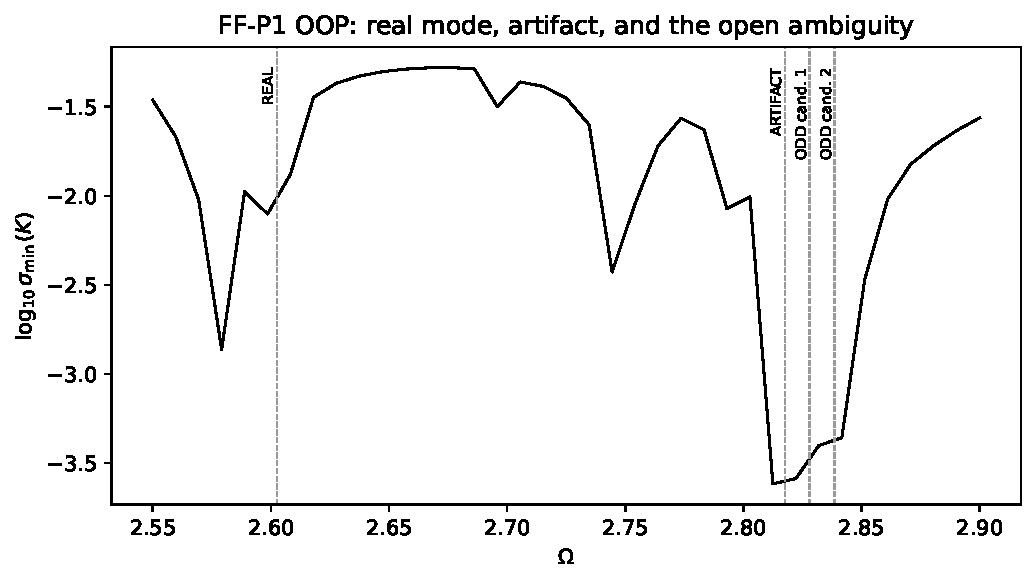
\includegraphics[width=0.50\linewidth]{sigmin_trace_2p55_2p90}\\[-0.15em]
{\footnotesize (a) $\sigma_{\min}$ trace, raw $[2.55,2.90]$}\\[0.2em]
\begin{minipage}{0.20\linewidth}\centering
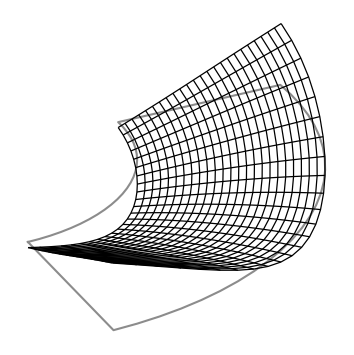
\includegraphics[width=\linewidth]{modeshape_phys_fundamental_tight}\\[-0.08em]
{\footnotesize (b) physical, $\Omega=0.383695$}
\end{minipage}\hfill
\begin{minipage}{0.20\linewidth}\centering
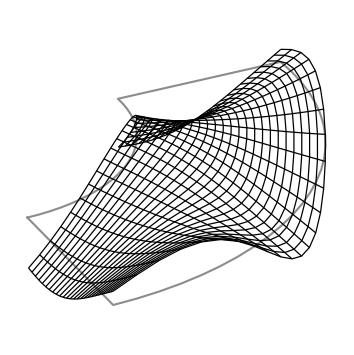
\includegraphics[width=\linewidth]{modeshape_phys_midspectrum_tight}\\[-0.08em]
{\footnotesize (c) physical, $\Omega=1.369611$}
\end{minipage}\hfill
\begin{minipage}{0.20\linewidth}\centering
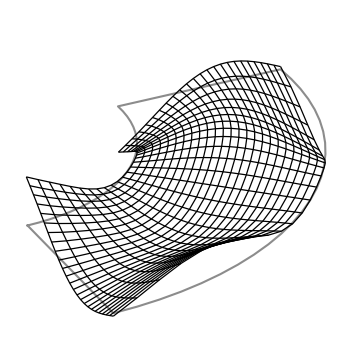
\includegraphics[width=\linewidth]{modeshape_phys_highest_tight}\\[-0.08em]
{\footnotesize (d) physical, $\Omega=2.602500$}
\end{minipage}\hfill
\begin{minipage}{0.20\linewidth}\centering
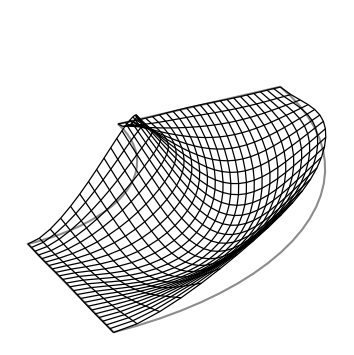
\includegraphics[width=\linewidth]{modeshape_artifact_even_2p8176_tight}\\[-0.08em]
{\footnotesize (e) spurious, $\Omega=2.817613$}
\end{minipage}
\caption{$\sigma_{\min}$ neighborhood of the EVEN artifact (a) and
reconstructed mode shapes at $n_{\mathrm{dofs}}=20$ (b--e). Panels
(b)--(d) are physical flexural modes; (e) is the displacement-free
spurious zero of \S5 ($r_M=75.52$). Unlabeled minima in (a) are
out-of-table-window or rejected scan features, not additional tabulated
modes.}
\label{fig:modeshapes}
\end{figure}

\section{Comparisons and tabulated frequencies}
A fully-default detector pass is not certified complete (\S4); the
tables in this section use the \S5 instruments. The flexural and
extensional tables are not the same evidence class and are not labeled
by a single word. Flexural frequencies
(\S6.2--\S6.3) are compared to mesh-converged FE under a two-sided,
portable residual screen; their only independent published check is
at a different radius ratio (\S\ref{sec:shi2014oop}: 6 of 6
refined roots). Extensional frequencies (\S6.3, \S\ref{sec:wang},
\S\ref{sec:qin}) are compared to FE \emph{and} to two published
semi-analytical tables, but only under a one-sided, geometry-specific
adjudication: there is no portable in-plane \emph{residual} bar. A
two-sided bar on mode-shape correlation is established separately in
\S\ref{sec:ipmacbar}; tabulated residual ratios are unchanged. That bar
is used in \S\ref{sec:r200a100} to resolve eight residual-unresolved
candidates at a second radius ratio, and in \S\ref{sec:ipmacbar} on all
24 extensional keys of the geometry sweep. A second, FE-free two-sided
bar (SUBDOM) is established in \S\ref{sec:subdom}: it certifies a root
from the boundary determinant alone. The cantilever
replication (\S6.1) is a third class: agreement with tables published
before this implementation existed. \S6.2 uses the orthotropic material
of Shi, Liang, Wang and Teng \cite{shi2016} in an independently-run FE model,
not their printed free-free row.

Table~\ref{tab:roadmap} maps every geometry treated below to what it was
checked against and the headline result, before the subsections that
follow work through each one.

\begin{table}[!htb]\centering\scriptsize
\caption{Validation roadmap: every geometry/motion pair, what it is
checked against, and the headline result. FE~= independently-run
mesh-converged finite-element model (\S6.2--\S6.5); lit.\ =
independently published table, matched directly
(\S6.1 and \S\ref{sec:wang}--\S\ref{sec:shi2014oop}).
One-to-one = every candidate individually cross-matched to an FE mode;
raw rate = nearest-neighbor FE-match fraction; MAC = the two-sided
mode-shape bar of \S\ref{sec:ipmacbar}. $\nu=0.30$ except the
24-geometry sweep and the extensional MAC sweep (both $\nu=0.35$).
$^{*}$one-to-one matching does not mean every target has its own
distinct root (see text).}
\label{tab:roadmap}
\begingroup
\renewcommand{\arraystretch}{0.88}
\setlength{\tabcolsep}{3pt}
\newcolumntype{L}{>{\raggedright\arraybackslash\hsize=.55\hsize}X}
\newcolumntype{H}{>{\raggedright\arraybackslash\hsize=1.45\hsize}X}
\begin{tabularx}{\linewidth}{@{}lLlllH@{}}
\toprule
\S & $R_i/R_o$, $2\Theta/\pi$ & Motion & Checked against & Standard & Headline result\\
\midrule
6.1 & annular cantilever (8 OOP + 3 IP geometries) & OOP+IP & \cite{seok1,seok2} (lit.) & one-to-one & all 29 published entries reproduced\\
6.2 & 0.5, 0.5 (orthotropic) & OOP & FE & one-to-one & 8/8, max err 1.08\%\\
6.3 & 0.5, 0.5 (primary) & OOP & FE & one-to-one & 8/8, max err 0.64\%\\
6.3 & 0.5, 0.5 (primary) & IP & FE & one-to-one$^{*}$ & 26 roots cover 27 FE modes, worst 0.052\%\\
6.4 & 0.500--0.667 $\times$ 6 angles & OOP+IP & FE & raw rate & 1256/1475 (85.2\%) within 3\%\\
6.5 & 0.5, 1.0 & OOP & FE & one-to-one & 15/15 ($\nu{=}0.30$) + 14/14 ($\nu{=}0.35$) REAL-like\\
6.5 & 0.5, 1.0 & IP & FE & raw rate & 61/64 ($\nu{=}0.30$), 57/61 ($\nu{=}0.35$)\\
6.5 & 0.6, 1.0 & OOP & FE & one-to-one & 18/18 REAL-like, all FE-matched\\
6.5 & 0.6, 1.0 & IP & FE & raw rate & 68/75 (90.7\%)\\
6.5 & 0.6, 0.5 & OOP & FE & one-to-one & 10/10 REAL-like, all FE-matched\\
6.5 & 0.6, 0.5 & IP & FE & raw rate & 43/47 (91.5\%)\\
6.6 & 3 geometries + 24-key sweep & IP & FE eigenvectors & MAC & every candidate separated (0.744)\\
6.7 & 4 geometries + full blind set & IP & none (FE-free) & angle/SUBDOM & 50/50 curated; 70/77 blind, 73 after 3 corrected pairings\\
6.8 & 0.5, 1.0 (orthotropic) & IP & \cite{wangip2016} (lit.) & one-to-one & 8/8, max err 0.649\%\\
6.9 & 0.5, 0.5 (primary) & IP & \cite{qin2018} (lit.) & one-to-one$^{*}$ & all 6 published values accounted for\\
6.10 & 0.4, 0.5 & OOP & \cite{shi2014sector} (lit.) & one-to-one & 6/6 refined roots, worst 0.149\%\\
\bottomrule
\end{tabularx}
\endgroup
\end{table}

\subsection{Cantilever replication}
The implementation reproduces the tabulated frequencies of
\cite{seok1,seok2}. The solver-computed side of this comparison
(Table~\ref{tab:cantilever-oop}, Table~\ref{tab:cantilever-ip}) was
regenerated from scratch under the deployed
\texttt{SOLVER\_VERSION} \texttt{2026-07-10.s10}, one geometry per task,
with no value carried over from an earlier capture: every published entry
matches, to $1.23\%$ out-of-plane and $1.39\%$ in-plane.

\begin{table}[!htbp]
\centering
\begin{minipage}[t]{0.49\textwidth}
\centering\scriptsize
\setlength{\tabcolsep}{2.6pt}
\captionsetup{width=\linewidth,justification=raggedright,singlelinecheck=false}
\caption{Cantilever replication, OOP vs.\ \cite{seok1}.}
\label{tab:cantilever-oop}
\begin{tabular}{cccccc}
\toprule $r_0/(2b)$ & $2\Theta/\pi$ & Mode & Computed & Paper & Err (\%)\\ \midrule
1.25 & 0.25 & 1 & 0.345324 & 0.341120 & 1.232\\
1.25 & 0.25 & 2 & 1.018530 & 1.013440 & 0.502\\
1.25 & 0.25 & 3 & 1.722434 & 1.718720 & 0.216\\
1.25 & 0.50 & 1 & 0.099419 & 0.099060 & 0.363\\
1.25 & 0.50 & 2 & 0.343742 & 0.340670 & 0.902\\
1.25 & 0.50 & 3 & 0.605904 & 0.604220 & 0.279\\
1.25 & 0.75 & 1 & 0.050717 & 0.050830 & 0.221\\
1.25 & 0.75 & 2 & 0.151458 & 0.149870 & 1.060\\
1.25 & 0.75 & 3 & 0.376503 & 0.376280 & 0.059\\
1.25 & 1.00 & 1 & 0.033153 & 0.033220 & 0.201\\
1.25 & 1.00 & 2 & 0.080358 & 0.079770 & 0.738\\
1.25 & 1.00 & 3 & 0.243521 & 0.243120 & 0.165\\
1.25 & 1.25 & 1 & 0.024652 & 0.024640 & 0.048\\
1.25 & 1.25 & 2 & 0.049473 & 0.049340 & 0.269\\
1.25 & 1.25 & 3 & 0.151555 & 0.151160 & 0.261\\
1.25 & 1.50 & 1 & 0.019790 & 0.019730 & 0.305\\
1.25 & 1.50 & 2 & 0.034523 & 0.034550 & 0.078\\
1.25 & 1.50 & 3 & 0.097470 & 0.097260 & 0.216\\
5/3 & 1.00 & 1 & 0.018023 & 0.018050 & 0.148\\
5/2 & 1.00 & 1 & 0.007762 & 0.007770 & 0.102\\ \bottomrule

\end{tabular}
\end{minipage}\hfill
\begin{minipage}[t]{0.49\textwidth}
\centering\scriptsize
\setlength{\tabcolsep}{2.6pt}
\captionsetup{width=\linewidth,justification=raggedright,singlelinecheck=false}
\caption{Cantilever replication, IP vs.\ \cite{seok2}.}
\label{tab:cantilever-ip}
\begin{tabular}{cccccc}
\toprule $r_0/(2b)$ & $2\Theta/\pi$ & Mode & Computed & Paper & Err (\%)\\ \midrule
1.25 & 0.25 & 1 & 0.341243 & 0.345890 & 1.343\\
1.25 & 0.25 & 2 & 0.808929 & 0.819210 & 1.255\\
1.25 & 0.25 & 3 & 0.940032 & 0.940120 & 0.009\\
1.25 & 0.50 & 1 & 0.120677 & 0.120880 & 0.168\\
1.25 & 0.50 & 2 & 0.347033 & 0.351910 & 1.386\\
1.25 & 0.50 & 3 & 0.529239 & 0.529300 & 0.012\\
1.25 & 1.00 & 1 & 0.039466 & 0.039480 & 0.035\\
1.25 & 1.00 & 2 & 0.106529 & 0.105560 & 0.918\\
1.25 & 1.00 & 3 & 0.263049 & 0.261290 & 0.673\\ \bottomrule

\end{tabular}
\end{minipage}
\end{table}
The largest out-of-plane residual is $1.23\%$, at the narrowest sector
$2\Theta/\pi=0.25$; the thin-ring row $r_0/(2b)=5/2$, where the source
papers reported slower convergence, agrees to $0.10\%$.
The cantilever table does not contain the
primary free-free geometry ($r_0/(2b)=1.5$, $2\Theta/\pi=0.5$); the
nearest tabulated rows are $r_0/(2b)=1.25$, $2\Theta/\pi=0.50$
(0.28--0.90\%) and $r_0/(2b)=5/3$ (0.15\%). Supplementary
Table~S.1 shows all eight free-free flexural labels move by less than
0.18\% from $n=20$ to $n=36$, so the 0.64\% FE residual of
Table~\ref{tab:oop} is larger than the documented basis-size movement at
this geometry. Several extensional labels in Table~S.2 move by 0.1--0.5\%
with basis size, which exceeds the 0.052\% FE residual of
Table~\ref{tab:ip}: that residual is a match to FE, not a claim that the
tabulated in-plane digits have converged to 0.05\%.
\subsection{Orthotropic free-free (ANSYS finite-element benchmark)}
The benchmark configuration is a completely free orthotropic annular
sector, radius ratio $R_i/R_o=0.5$, sector angle $2\Theta=\pi/2$, using the
orthotropic material adapted from Shi, Liang, Wang and Teng \cite{shi2016}
(\S\ref{sec:ortho}). Targets are an independently-run, mesh-converged
ANSYS \cite{ansys} SHELL281 model of this same geometry and material
($64\times64$/$96\times96$ refinements, $<0.01\%$ agreement), not values
transcribed from a published table. \cite{shi2016} specify
$E_r=40E_\theta=2800$~GPa; the value solved here, $E_r=40$~GPa, is a
different material, identified as such only after this benchmark was
built, and no agreement with their printed free-free row is claimed. The
reduction formulae of \S\ref{sec:ortho} are separately checked against a
published orthotropic table in \S\ref{sec:wang}, 8 of 8 to $0.649\%$.
All 8 targets match (Table~\ref{tab:shi}).

\begin{table}[h]\centering\small
\caption{Orthotropic free-free flexural modes vs.\ ANSYS
($\Omega_{\mathrm{lit}}$; orthotropic material adapted from
Shi, Liang, Wang and Teng \cite{shi2016}, \S\ref{sec:ortho}).
Max err $1.08\%$; isotropic counterpart is Table~\ref{tab:oop} ($0.64\%$).
Conversion constants $T=0.672859$, $R^{*}=1.75$, $\mu_\theta=0.525$.}
\label{tab:shi}
\begin{tabular}{ccc}
\toprule FEM & Solver ($\Omega_{\mathrm{lit}}$) & err (\%)\\ \midrule
12.40 & 12.5335 & 1.08\\
15.57 & 15.6298 & 0.38\\
36.13 & 36.3107 & 0.50\\
43.65 & 43.8826 & 0.53\\
66.76 & 67.2235 & 0.69\\
87.46 & 88.0668 & 0.69\\
89.82 & 90.3233 & 0.56\\
95.35 & 96.0312 & 0.71\\
\bottomrule
\end{tabular}
\end{table}
\subsection{Isotropic free-free vs.\ finite elements}
Table~\ref{tab:oop} and Table~\ref{tab:ip} report frequency in two
different conventions, not a single shared unit: the flexural table
converts to the classical literature ratio $\Omega_{\mathrm{lit}}$
(\S3.1; Supplementary Material, §S.3.6) to match Shi, Liang, Wang and
Teng's and the original Seok--Tiersten convention, while the extensional
table reports the raw solver $\Omega$ directly against FE frequency in
Hz, since $\Omega$ is already the correct in-plane ratio with no further
conversion. The two columns are not directly comparable.
Benchmarks are mesh-converged ANSYS models, with a half-sector
symmetric/antisymmetric study certifying each benchmark mode's parity.
The flexural benchmark uses SHELL281 shell elements in a two-pass deck at
$64\times64$ and $96\times96$ divisions, with matched elastic modes
required to agree to $<0.3\%$ between the two meshes before use; the
realized agreement is far tighter, the eight tabulated flexural modes
differing by at most $1.5\times10^{-4}\%$ between the two passes. Because a
free-free shell model interleaves the flexural, extensional, and
rigid-body families in one spectrum, the numerically-zero rigid modes are
discarded and extensional-family modes are identified and removed by
frequency-matching against the companion plane-stress model. The
extensional benchmark itself is that PLANE183 plane-stress model, built as
the same two-pass $64\to96$ refinement and held to the same standard, with
a realized worst-case difference of $5.8\times10^{-4}\%$ over the 27
elastic modes below 1120~Hz. Both convergence passes are contained in the
released ANSYS output files, so either figure can be recomputed directly.

One systematic difference between the two sides sets a floor on the
agreement reported below and is worth naming. SHELL281 is a first-order
shear-deformable element; the present solution is classical Kirchhoff
(\S3.1). Shear flexibility and rotary inertia lower a finite-element
frequency relative to a Kirchhoff one by roughly
$\tfrac12\big[Dk^2/(\kappa GH)+k^2H^2/12\big]$ at effective bending
wavenumber $k$ ($\kappa=5/6$, $G$ the shear modulus), which for this plate
is $0.03\%$ at the first tabulated flexural mode rising to $0.19\%$ at the
eighth. That is the right sign in every row --- the solver sits above FE in
all eight rows of Table~\ref{tab:oop} and all eight of
Table~\ref{tab:shi} --- and the right order of magnitude, so part of the
one-sided residual reported below is a difference between two plate
theories rather than error in either. The one comparison in this paper
against a solution built on that same classical theory
(\S\ref{sec:shi2014oop}, Shi et al.'s thin-plate Fourier-series annular
sector table) agrees an order of magnitude more tightly,
$0.002$--$0.149\%$, and is not one-signed.

Rigid-body modes (one transverse translation and two rotations for
flexural motion; two in-plane translations and one rotation for
extensional motion) occur at zero frequency for the completely free
plate, lie below every scanned frequency window, and are excluded from
all mode counts and matching on both the solver and FE sides: mode~1 in
every table is the first elastic mode, following the literature
convention.
Table~\ref{tab:oop} lists the physical flexural matches, all
$\le 0.64\%$; the rejected zeros are Supplementary Material, Table~S.8
(the last row is Fig.~\ref{fig:modeshapes}(e)). Extensional: 26 distinct
solver roots (Table~\ref{tab:ip}); 25 of the 27 extensional FE modes
below 1120~Hz have a unique partner (worst 0.052\%); the FE pair at
459.5/460.6~Hz is split by the solver (0.006\% each) while the pair at
1114.9/1115.3~Hz is one production-detector root, so 27 FE frequencies
are accounted for, not 27 independent assignments.\footnote{An isolated
refinement finds two distinct, shift-stable roots underneath this one
production singularity, each within $0.015\%$ of one FE member; MAC
against both shows they are the \emph{same} shape (one shape, two
frequencies), so the single-root table entry is correct as tabulated,
not a missed split. Full resolution, including the isolated frequencies
and MAC values: Supplementary Material, §S.3.4.}
Table~\ref{tab:oop} reports raw $\bar k\bar\Omega$, not $\Omega$;
Table~\ref{tab:ip}'s raw column is the plain
$\Omega=\omega/\bar\omega$ (\S3.1).

\begin{table}[!htbp]\centering\footnotesize
\caption{Free-free flexural modes vs.\ FEM ($\Omega_{\mathrm{lit}}$).
Depth is $\log_{10}\sigma_{\min}$ at the $n{=}20$ screening basis of \S5.}
\label{tab:oop}
\begin{tabular}{cccccc}
\toprule Raw $\bar k\bar\Omega$ & $f$(Hz) & Solver ($\Omega_{\mathrm{lit}}$) & FEM & err (\%) & depth\\ \midrule
0.383695 & 4.732 & 15.148 & 15.128 & 0.13 & $-3.42$\\
0.616645 & 7.605 & 24.344 & 24.190 & 0.64 & $-3.91$\\
0.961312 & 11.855 & 37.951 & 37.818 & 0.35 & $-3.69$\\
1.369611 & 16.890 & 54.070 & 53.828 & 0.45 & $-4.78$\\
1.752188 & 21.608 & 69.174 & 68.847 & 0.47 & $-3.91$\\
2.320741 & 28.620 & 91.619 & 91.452 & 0.18 & $-2.81$\\
2.379886 & 29.349 & 93.954 & 93.537 & 0.45 & $-4.21$\\
2.602500 & 32.095 & 102.743 & 102.136 & 0.59 & $-3.70$\\ \bottomrule
\end{tabular}
\end{table}

\begin{table}[!htb]\centering\scriptsize
\caption{Free-free extensional modes: raw $\Omega$ vs.\ FEM.
Twenty-six distinct solver roots; 25 FE modes have a unique partner.
Entry 26 also matches the 1115.3~Hz partner, so 27 FE frequencies are
accounted for, not 27 independent assignments (\S6.3). Raw column is not comparable to
Table~\ref{tab:oop} (\S3.1).}
\label{tab:ip}
\begin{tabular}{cccc|cccc}
\toprule \# & $\Omega$ & FEM $f$(Hz) & err(\%) & \# & $\Omega$ & FEM $f$(Hz) & err(\%)\\ \midrule
1 & 0.401154 & 161.4 & 0.025 & 14 & 1.832694 & 736.8 & 0.052\\
2 & 0.687446 & 276.5 & 0.007 & 15 & 1.972966 & 793.6 & 0.001\\
3 & 0.764697 & 307.5 & 0.030 & 16 & 1.987180 & 799.3 & 0.003\\
4 & 1.142287 & 459.5 & 0.006 & 17 & 1.996235 & 803.0 & 0.004\\
5 & 1.145158 & 460.6 & 0.006 & 18 & 2.166815 & 871.6 & 0.002\\
6 & 1.197600 & 481.7 & 0.005 & 19 & 2.293214 & 922.3 & 0.013\\
7 & 1.416689 & 569.7 & 0.026 & 20 & 2.301512 & 925.7 & 0.007\\
8 & 1.440568 & 579.3 & 0.027 & 21 & 2.389113 & 960.7 & 0.031\\
9 & 1.522330 & 612.3 & 0.007 & 22 & 2.450795 & 985.7 & 0.011\\
10 & 1.598985 & 643.1 & 0.012 & 23 & 2.521489 & 1014.1 & 0.014\\
11 & 1.613123 & 648.8 & 0.010 & 24 & 2.566362 & 1032.0 & 0.029\\
12 & 1.690020 & 679.8 & 0.001 & 25 & 2.676026 & 1075.9 & 0.047\\
13 & 1.779792 & 715.9 & 0.001 & 26 & 2.771955 & 1114.9 & 0.008\\
\bottomrule
\end{tabular}

\vspace{0.25em}
{\footnotesize Raw column is $\Omega=\omega/\bar\omega$, not
$\bar k\bar\Omega$; not comparable to Table~\ref{tab:oop} (\S3.1).}
\end{table}

The extensional count above does not include the flexural FE mode at
$\Omega_{\mathrm{lit}}=111.46$, which lies above Table~\ref{tab:oop}'s
window and is left as an open assignment: the solver has two ODD-parity
dips, at raw 2.828013 (0.16\% from the FE value) and raw 2.838515
(0.54\% away). An eight-instrument suite fails to force an assignment
between them; the individual instruments and their outcomes are in
Supplementary Material, §S.3.2. The decisive instrument is MAC: alone among the eight, it judges mode \emph{shape} instead of frequency or matrix structure. Both candidates reconstruct as genuinely ODD-parity and
correlate almost perfectly with the FE eigenvector (cand.\ 2.828013:
MAC $=0.9913$; cand.\ 2.838515: MAC $=0.9999$), a gap of only 0.0086
against the $0.2$ forced-call threshold used here, more conservative
than the conventional experimental-modal bands of
Ref.~\cite{allemang2003} ($0.9$/$0.05$ good/uncorrelated). Two further,
independent checks (basis-size stability and an independent
pure-slope-residual comparison; Supplementary Material, §S.3.2) confirm
both are radially distinct, genuine modes, not one a numerical echo of
the other. Both are therefore confirmed genuine, high-fidelity
ODD-parity modes; the FE mode is not missing from the solver spectrum,
and the pair is best interpreted as a real, basis-independent
near-degenerate pair ($\Delta\Omega\approx0.0105$, ${\sim}$0.4\% apart)
whose mode shapes are too similar for any instrument to separate; the
assignment is left unforced, not resolved. Candidate 2.828013's
self-parity is basis-sensitive beyond the calibrated range
(Supplementary Material, §S.3.2).

\subsection{Geometry generalization: radius ratio and sector angle sweep}\label{sec:geomsweep}
Tables~\ref{tab:oop} and~\ref{tab:ip} validate the free-free detector at a
single geometry. To check how broadly that agreement generalizes, a second, independent sweep was run over 4 radius ratios ($R_i/R_o=0.500$--$0.667$) $\times$ 6 sector
angles ($\Theta=22.5^\circ$--$135^\circ$) --- 24 geometries, each run for
both motion types, so 48 geometry/motion combinations --- each run through the full solver pipeline
against an independent FE benchmark (a matching pair of ANSYS SHELL281/
PLANE183 models per geometry, same two-mesh convergence standard as
\S6.2) at a second isotropic material ($\nu=0.35$, so this is a
generalization check against its own FE ground truth, not a
re-validation of the $\nu=0.30$ geometry above).

Matching is nearest-neighbor, a coarser adjudication than
Tables~\ref{tab:oop}--\ref{tab:ip}'s one-to-one, parity-checked
assignment: no per-mode FE partner is claimed. The \S5 residual screen
was applied to every accepted flexural candidate (695 targets across
the 24 OOP geometry keys)\footnote{Job-level detail: Supplementary
Material, §S.3.3.}: 654 reconstructed
at the production basis, 329 REAL-like / 321 ARTIFACT-like /
4 AMBIGUOUS. The REAL-like fraction is $50.3\%$ over all 654 --- $47.9\%$
over the 119 cut-off-adjacent candidates among them against $50.8\%$ over
the other 535 --- so the calibrated flexural bar travels and does not
degrade near the cut-off.
The 41 reconstruction failures are the known even-valued
basis-fill shortfall, 33 of them at
$r_0/2b=2.5$, $2\Theta/\pi\le0.5$. Extensional candidates have no
portable verdict bar on the residual
(\S5, \S\ref{sec:r200a100}); the mode-shape bar of \S\ref{sec:ipmacbar}
was applied to all 24 extensional keys of this sweep at the sweep
material $\nu=0.35$. Setting aside a known cut-off-adjacent subset
with elevated error (consistent with the near-cutoff conditioning
behavior already noted in \S5), agreement is close and
geometry-independent: 1256 of 1475 candidates (85.2\%) matched an
independent FE mode within 3\%, mean of per-geometry mean errors 0.574\%,
with no degradation trend as $R_i/R_o$ increases (Supplementary Material,
Table~S.3). The $3\%$ window measures coverage, not precision, and on a
spectrum this dense it is loose: a frequency drawn uniformly across a
geometry/motion pair's own FE span lands within $3\%$ of \emph{some} FE
mode about $60\%$ of the time, so the hit rate alone sits only modestly
above chance.\footnote{Monte-Carlo estimate over each pair's own FE span,
using the FE modes that appear as a match in the shipped consolidated
manifest --- 889 of the 1517 modes actually extracted, so the true chance
rate is higher still.} What is not near chance is how close the matches
are: matched candidates' errors have median $0.315\%$, with $63.5\%$ inside
$0.5\%$ and $77.7\%$ inside $1\%$, against a median near $1.5\%$ for a
uniform draw in the same window. The precision of the agreement, not its
coverage, is what this sweep shows. The per-candidate set churned substantially under the
completeness work between checkpoints; 85.2\% is a re-derivation of the
aggregate, not an unchanged candidate list.\footnote{Superseded intermediate-recapture figures and full provenance: Supplementary Material, §S.3.3, §S.4.} This does not
replace Tables~\ref{tab:oop}--\ref{tab:ip} as the primary tabulated
comparison.
Coarse nearest-neighbor agreement is geometry-independent; full
residual-screened adjudication has been performed at four geometries.

\subsection{Mode-by-mode adjudication at three further geometries}
\label{sec:r150a100}\label{sec:r200a100}\label{sec:r200a50}
The sweep above is nearest-neighbor against FE and uses $\nu=0.35$.
The mode-by-mode standard of Tables~\ref{tab:oop} and~\ref{tab:ip} is
applied here at three further geometries that close the
$\{R_i/R_o=0.5,\,0.6\}\times\{2\Theta=\pi/2,\,\pi\}$ rectangle at
$\nu=0.30$ (the first of them also at $\nu=0.35$), each through the
same default production pipeline, one-to-one FE cross-match, and
\S5 residual/parity screen. Per-mode outcomes are Supplementary
Material, Tables S.4--S.6.

\begin{center}\footnotesize
\begin{tabular}{@{}llc>{\raggedright\arraybackslash}p{0.32\linewidth}@{}}
\hline
$R_i/R_o$, $2\Theta/\pi$ & OOP REAL-like & IP (raw) & distinctive finding \\
\hline
$0.5$, $1.0$ & $15/15$ ($\nu{=}0.30$) + $14/14$ ($\nu{=}0.35$)
  & $61/64$, $57/61$ & unmatched flexural candidates ARTIFACT-like only \\
$0.6$, $1.0$ & $18/18$, all $\le 0.62\%$
  & $68/75$ & residual populations overlap; FE\#23 unmatched \\
$0.6$, $0.5$ & $10/10$, all $\le 0.58\%$
  & $43/47$ & those 10 cover every in-range elastic FE mode \\
\hline
\end{tabular}
\end{center}

\noindent At every geometry, every REAL-like flexural candidate matched
an independent FE mode: no catalogued spurious zero passed the screen at
any of the three. The converse does not hold everywhere --- one in-range
FE mode at $(0.6,\,1.0)$ has no REAL-like partner, below --- so what these
geometries establish is that the screen's REAL-like calls are reliable,
not that its coverage of the FE spectrum is complete. Errors again fall on
one side only, the same pattern as Table~\ref{tab:oop}. Unmatched flexural
candidates are ARTIFACT-like, concentrated in near-degenerate
neighborhoods of the kind documented for the ODD pair (\S6.3), and are
not force-assigned.

The first geometry isolates sector angle at the primary radius ratio
($R_i/R_o=0.5$, $2\Theta/\pi=1.0$, a half-annulus against the primary
quarter-annulus). Raising the FE extract from 35 to 80 modes recovered
every extensional candidate that had sat above the old ${\sim}798$~Hz
ceiling; the few remaining non-matches all lie below that ceiling and
are residual-classified ARTIFACT-like or AMBIGUOUS.

The second isolates radius ratio at that new angle
($R_i/R_o=0.6$, $2\Theta/\pi=1.0$). One in-range FE mode has no
production-capture partner (FE mode 23 of 34,
$\Omega_{\mathrm{lit}}=129.650$); FE mode 9
($\Omega_{\mathrm{lit}}=16.100$) is a second root next to the FE\#10
partner, missed at $n{=}20$ because the dip sat just short of the
$-3.5$ accept floor.\footnote{At $n{=}28$ and $n{=}36$,
$\Omega^{*}=0.261289$ ($\Omega_{\mathrm{lit}}=16.1176$, err $0.109\%$,
depths $-6.74$ and $-6.43$, shift $0.0002\%$, $2.17\%$ from the claimed
neighbor $0.267076$). FE\#23 had no second minimum in the unconstrained
scan. Job-level detail: Supplementary Material, §S.4.}
Neither disturbs the property above: every REAL-like call at this
geometry still has its own FE partner. This geometry also shows why no extensional
\emph{residual} bar is claimed. Restricting to the 74 candidates below
the FE extraction ceiling, and taking a match within $0.5\%$ as
presumptive-physical and the absence of any match within $3\%$ as
presumptive-spurious, the two populations do not separate:
$r_{\theta\theta}=0.009$--$7.6$ against $2.8$--$9.6$. None of the
presumptive-spurious candidates falls below $0.349$, the largest REAL-like
reading on the primary geometry's complete set when every candidate is
evaluated at its own converged root (\S5; that same set read at its
catalogued seeds on the owning block reaches $0.6858$, Supplementary
Material, Table~S.7), while 34 of 49 presumptive-physical ones do: a low residual
is evidence of a physical mode here, a high one is not evidence
against. Eight candidates match an FE mode tightly while reading above
the spurious group's lower edge; scored on the mode-shape bar of
\S\ref{sec:ipmacbar}, six are ARTIFACT-like (same-class MAC
$0.18$--$0.58$) and two are REAL-like ($\Omega=1.667187$ against FE\#33,
MAC $0.9981$; $\Omega=1.894176$ against FE\#42, MAC $0.9953$). For four
of the six artifacts the nearest-frequency FE target belongs to the
opposite symmetry class, so MAC against that target is identically
zero. A tight frequency match at this geometry is not by itself
evidence of a physical mode.

The third geometry crosses the two axes ($R_i/R_o=0.6$,
$2\Theta/\pi=0.5$). The ten REAL-like roots cover every in-range
elastic FE mode (FE modes 7--16 of 34). FE mode 16 is also claimed by
an ARTIFACT-like companion ($\Omega=2.412108$, $1.86\%$), the same
near-degenerate pairing as \S6.3, not force-assigned. Unlike the
second geometry, no in-range flexural FE mode lacks a REAL-like
partner. The four extensional misses are residual-classified
ARTIFACT-like.

That closes the $\{R_i/R_o=0.5,\,0.6\}\times\{2\Theta=\pi/2,\,\pi\}$
rectangle at $\nu=0.30$. It does not make the 24-geometry sweep
one-to-one, and it does not supply a portable extensional bar on the
residual; for a two-sided bar on mode-shape correlation see
\S\ref{sec:ipmacbar}.

\subsection{A portable two-sided extensional bar on mode-shape
correlation}\label{sec:ipmacbar}
Every tabulated extensional frequency above is still residual-adjudicated:
no portable two-sided bar exists on the pointwise edge residual, and none
is claimed. A different instrument does supply one. The eight candidates
of \S\ref{sec:r200a100} are scored on it. The modal assurance criterion (MAC) already used
in \S6.3 to resolve the flexural ceiling ambiguity draws on mode \emph{shapes} rather than boundary residuals, so it is structurally independent of the quantity that fails to port.
Throughout this subsection MAC is the identity-weighted correlation of
the stacked nodal in-plane displacement $(U_X,U_Y)$, not a mass-weighted
form: if $\mathbf{a}$ and $\mathbf{b}$ are the two stacked vectors,
$\mathrm{MAC}=|\mathbf{a}\cdot\mathbf{b}|^2/(\|\mathbf{a}\|^2\|\mathbf{b}\|^2)$.
Production scoring takes the maximum of that quantity over FE modes of
the same symmetry class as the root-owning block. The production call is
the midpoint $0.744$ of the $\nu=0.30$ calibration window below. Building
$\mathbf{a}$ requires evaluating the exact reconstruction at each FE
node's coordinates and resolving the two models' angular origins;
Supplementary Material, §S.3.2 gives that procedure,
including the mesh-pairing step it depends on for classifying FE modes
by symmetry (exact at $2\Theta=\pi$; a Cartesian-midside fallback at
every other sector angle, including the primary $2\Theta=\pi/2$).
A MAC taken across parity blocks is analytically zero, so each
candidate is scored on the block that owns a root at its own $\Omega$
(Supplementary Material, §S.3.2).

Scored that way, MAC separates the two populations at all three
fully-adjudicated geometries, on the same already-published REAL-like /
ARTIFACT-like calibration sets used elsewhere in this paper: eight
candidates per geometry, four already labeled REAL-like and four
ARTIFACT-like by the residual screen or (for $r_0/2b=2.0$) by prior
one-to-one FE adjudication. At the primary geometry the REAL-like half
is drawn from Table~\ref{tab:ip}'s own published roots; the
ARTIFACT-like half are catalogued spurious zeros of the same
determinant, now listed with their owning-block residuals in
Supplementary Material, Table~S.7 (the in-plane analogue of
Table~S.8). The two
non-primary geometries' calibration sets are their own independently
adjudicated candidates, not rows of Table~\ref{tab:ip}, which covers
only $r_0/2b=1.5$, $2\Theta/\pi=0.5$.

\begin{center}\footnotesize
\begin{tabular}{lccc}
\hline
geometry ($r_0/2b$, $2\Theta/\pi$) & $\min(\mathrm{MAC_{REAL}})$ &
$\max(\mathrm{MAC_{ART}})$ & gap \\
\hline
$(1.5,\,0.5)$ & 0.9079 & 0.0067 & $+0.9012$ \\
$(2.0,\,1.0)$ & 0.9869 & 0.5801 & $+0.4068$ \\
$(2.0,\,0.5)$ & 0.9994 & 0.3480 & $+0.6514$ \\
\hline
\end{tabular}
\end{center}

\noindent Combined, with every candidate evaluated at its catalogued
frequency, the REAL floor is $0.9079$ and the ARTIFACT ceiling $0.5801$:
any threshold between them classifies all 24 candidates
correctly.\footnote{The three-geometry calibration table was
independently reproduced bit-for-bit against a transcribed gate table,
and each geometry reproduces its own previously-published per-block
residuals to $10^{-4}$ relative (job-level detail: Supplementary
Material, §S.4). Robustness of the reported window to the choice of
seed-versus-own-root evaluation and to the FE-target pairing rule is
established in Supplementary Material, §S.3.2.}
Local-minimum block selection, with residual tie-break, classifies
24 of 24; either simpler criterion alone is 23 of 24
(Supplementary Material, §S.3.2). Two candidates held out of the
calibration, where residual and FE disagree, both read MAC $0.998$ and
agree with the FE evidence.

Three limits bound the $\nu=0.30$ calibration. The bar is calibrated on
FE-matched Table~\ref{tab:ip} roots and independently adjudicated
ARTIFACT-like zeros (one of the four primary REAL seeds, row 23, sits in
the residual middle band; Supplementary Material, Table~S.7), so its
demonstrated added value is the tie-break above rather than a blind
re-adjudication. At $(2.0,\,0.5)$ all three
selection criteria score 8 of 8, so that geometry confirms the bar
transfers but supplies no evidence that the rule is better than the
simpler alternatives; the rule's margin rests on two candidates.
The ARTIFACT ceiling on that calibration set is strongly
geometry-dependent ($0.0067$, $0.3480$, $0.5801$). It is now the production
two-sided extensional classification instrument when FE eigenvectors are
available: local-minimum block selection, MAC scored as the maximum
over FE modes of the same symmetry class as the root-owning block,
threshold $0.744$. It is not inside the frequency detector and does not
change a computed $\Omega$. Tabulated residual ratios are unchanged.
\S\ref{sec:r200a100} reports the bar's call on the eight
residual-unresolved candidates at that geometry: six ARTIFACT-like, two
REAL-like.

The $\nu=0.30$ window $(0.5801,0.9079)$ is a calibration result; nothing
here claims it as a universal floor. The same production call was then applied to
every accepted extensional candidate at all 24 keys of the
\S\ref{sec:geomsweep} sweep, at that sweep's own material $\nu=0.35$,
against an independent PLANE183 extract of the same 57 elastic modes
(FE modes 4--60) used at the primary calibration geometry. The C-class rows at $2\Theta/\pi=1.25$
and $1.50$ have no tight MAC-REAL in that extract; repeating those eight
keys against an 80-elastic-mode extract still produced none
(Supplementary Material, §S.4).\footnote{Tight means an FE match
within $0.5\%$. Flexure on this sweep remains residual-screened; this is
the extensional MAC application, not a one-to-one residual adjudication
of the 24-geometry table.} Combined, all $1596$ extensional candidates the sweep produces
reconstructed (\S\ref{sec:geomsweep}'s $1475$ is the smaller subset left
after removing cut-off-adjacent and beyond-FE-range candidates from both
motion types; Supplementary Material, Table~S.3); $912$ match an FE mode within $0.5\%$, of which
$410$ are MAC-REAL and $502$ are MAC-ART at threshold $0.744$, with no
tight misclassification on either side of that threshold. The call splits
by sector angle, not by radius ratio. Each row below pools that angle's four
radius ratios, and its outcome column is the declared-before-pooling verdict class for
the angle: A where both populations are present and the threshold separates
them, C where the sweep produced no tight MAC-REAL candidate at any radius
ratio.

\begin{center}\footnotesize
\begin{tabular}{lcccccc}
\hline
$2\Theta/\pi$ & recon. & tight & REAL/ART &
$\min(\mathrm{MAC_{REAL}})$ & $\max(\mathrm{MAC_{ART}})$ & outcome \\
\hline
$0.25$ & 97/97 & 62 & 51/11 & 0.9547 & 0.6551 & A \\
$0.50$ & 163/163 & 101 & 78/23 & 0.8218 & 0.6650 & A \\
$0.75$ & 256/256 & 160 & 131/29 & 0.9260 & 0.5130 & A \\
$1.00$ & 303/303 & 187 & 150/37 & 0.8495 & 0.6803 & A \\
$1.25$ & 376/376 & 214 & 0/214 & --- & 0.5993 & C \\
$1.50$ & 401/401 & 188 & 0/188 & --- & 0.4295 & C \\
\hline
\end{tabular}
\end{center}

\noindent The sixteen keys with $2\Theta/\pi\le 1.0$ each have at least
one tight MAC-REAL and one tight MAC-ART. The eight keys at
$2\Theta/\pi=1.25$ and $1.50$ (every radius ratio) have none: every tight
FE-frequency match is MAC-ART, the same pattern seen among the eight
residual-unresolved candidates of \S\ref{sec:r200a100}. Because the two
C rows carry no REAL-side evidence, $0.744$ was left where the $\nu=0.30$
calibration had put it. Combined REAL floor on the sixteen keys that
have one is $0.8218$ ($r_0/2b=2.0$, $2\Theta/\pi=0.5$); combined ARTIFACT
ceiling is $0.6803$ ($r_0/2b=2.5$, $2\Theta/\pi=1.0$). Both sit inside
the $\nu=0.30$ calibration window: that window does not survive a change
of Poisson ratio, radius ratio, or sector angle, and the production
midpoint was not retuned. What travels is the call at $0.744$, which still splits every tight
candidate on all 24 keys. So a two-sided extensional bar does exist, with a
measured reach; it is simply not carried by the pointwise residual.

Figure~\ref{fig:macsummary} makes both tables above visible at a glance:
every calibration and sweep candidate's own MAC value against the
production threshold, rather than only the extrema. The two populations occupy
disjoint bands at every geometry; the closest approach from either side is
the $2\Theta/\pi=1.0$ sweep row's ARTIFACT ceiling of $0.6803$, still
$0.064$ clear of the threshold.
\begin{figure}[!htb]\centering
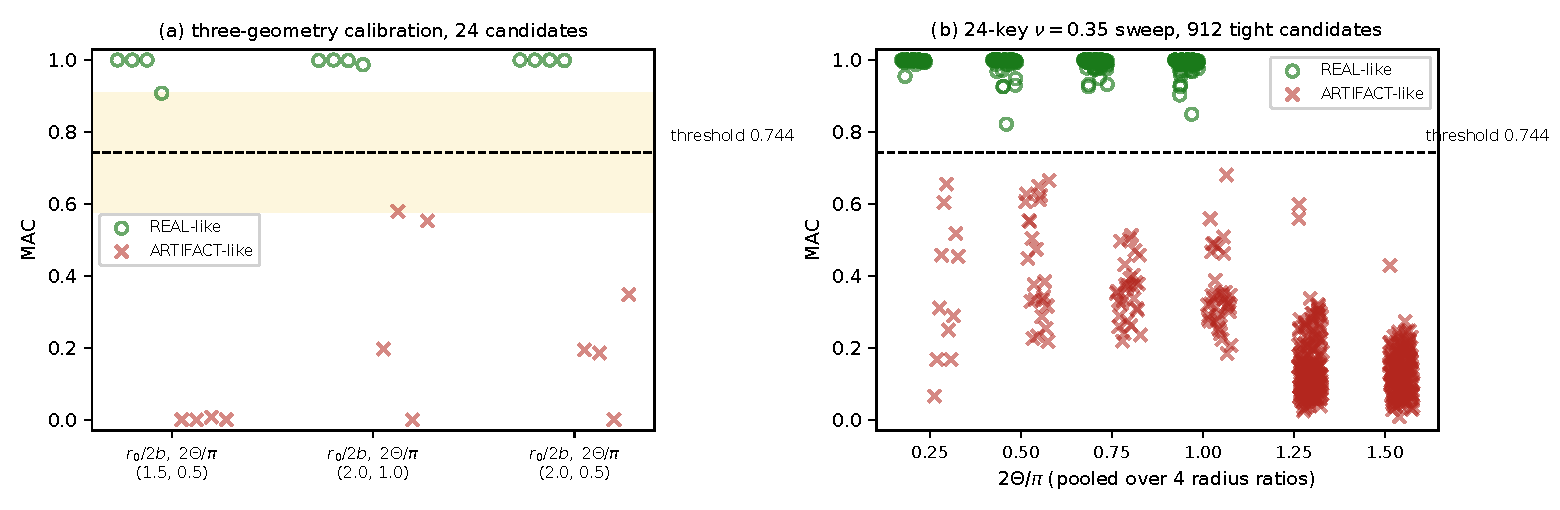
\includegraphics[width=\linewidth]{mac_separation_summary}
\caption{MAC separation of the two-sided extensional bar
(\S\ref{sec:ipmacbar}), REAL-like (green circles) vs.\ ARTIFACT-like (red
crosses) against the production threshold $0.744$ (dashed). (a) The
three fully-adjudicated calibration geometries of the (min REAL, max
ARTIFACT, gap) table above, every one of the 24 candidates individually
(not only the tabulated floor/ceiling); the shaded band is the combined
$\nu{=}0.30$ window $(0.5801,0.9079)$. (b) The 24-key $\nu{=}0.35$
geometry sweep of \S\ref{sec:geomsweep}, pooled by sector angle as in the
angle-pooled table above, every tight (FE match $<0.5\%$) candidate
individually; the $2\Theta/\pi=1.25,1.50$ keys have no REAL-like tight
candidate at all (\S\ref{sec:ipmacbar}), hence no green points in those
two columns.}
\label{fig:macsummary}
\end{figure}

\subsection{A finite-element-free two-sided extensional certification
criterion}\label{sec:subdom}
The mode-shape bar of \S\ref{sec:ipmacbar} closes the extensional
two-sidedness gap only where an FE eigenvector is available. A second,
independent instrument closes the same gap without one, certifying an
extensional root as real or spurious from the boundary determinant alone,
the way the flexural screen already does.

\paragraph{Construction.} This subsection introduces a small linear-algebra
notation; to keep it clear of the physical symbols of \S3, its matrices are
set in bold ($\mathbf{D},\mathbf{T},\mathbf{M},\mathbf{R}$, distinct from the
scalars $D$, $T$, $M_{r\theta}$, $R^{*}$), its traction-to-displacement ratio
is $\eta$ (never $\rho$, which is mass density throughout), and its pooling
factor is $\gamma$ (never $G$, which denotes a shear modulus elsewhere in
this paper). For extensional (in-plane) motion the same
boundary determinant that supplies $\mathbf{K}(\Omega)$ admits an exact
factorization $\mathbf{K}=\mathbf{D}^{\mathsf T}\mathbf{T}$, where $\mathbf{D}$
collects the displacement
weights and $\mathbf{T}$ the traction weights of the underlying two-edge
functional; the factorization was verified entrywise against the deployed
assembly (gate G1, bar $10^{-30}$, measured $1.21\times10^{-41}$ to
$8.80\times10^{-41}$). Define
$\eta(c)=\|\mathbf{T}c\|/\|\mathbf{D}c\|$ for a coefficient vector $c$, and
$\eta(\Omega)=\min_{c}\eta(c)$, the smallest traction-to-displacement
ratio attainable at that frequency. The deployed pointwise
residual screen of \S5 evaluates this ratio at one particular point, the
null vector of the accepted zero, $\eta(c_{\mathrm{null}})$;
since $c_{\mathrm{null}}$ is one feasible choice among all $c$,
$\eta(c_{\mathrm{null}})\ge\eta(\Omega)$
identically (gate G3), which is the algebraic source of that screen's
already-reported one-sidedness for extensional motion (\S5): a small
$\eta(c_{\mathrm{null}})$
certifies a physical root, but a large one does not certify an artifact,
because $\eta(\Omega)$ itself may still be small.

$\eta(\Omega)$ as a magnitude does not repair this: at the primary geometry the
REAL and ARTIFACT populations of $\eta(\Omega)$ overlap, and at $r_0/2b=2.0$,
$2\Theta/\pi=1.0$ the overlap is total. What separates the two populations
is not the minimizing ratio's \emph{size} but an \emph{angle}: at a
genuine root, $\mathbf{K}$'s null direction and the traction-minimizing direction
are the same physical displacement field; at a projection artifact they
are unrelated vectors that happen to share a small determinant. Two
refinements make that angle a working instrument. First, near-degenerate
directions must be pooled rather than compared one at a time: with
$\sigma_1\le\sigma_2\le\cdots$ the generalized singular values of the
whitened pencil ($\mathbf{D}=\mathbf{Q}\mathbf{R}$,
$\mathbf{M}=\mathbf{T}\mathbf{R}^{-1}$, SVD of $\mathbf{M}$), the criterion
projects onto the cluster of the
$p=\#\{i:\sigma_i\le\gamma\sigma_1\}$ lowest-traction
directions, with $\gamma=4$ the pooling value used in every result below.
$\gamma=3.0$ was the original pre-registered choice; the labelled sets already
showed the REAL/ARTIFACT separation stable across $\gamma=1.5$--$8$ before any
blind run, and a second-geometry blind set is inert for $\gamma=2$--$6$.
The one $\gamma=3.0$ miss in the first blind geometry (FE mode 23 below) sits
at a knife-edge $\gamma=3.01$; $\gamma=4$ is a round value inside that
pre-established window, not a fit to $3.02$. Second, the projection must be
taken on the \emph{interior} displacement field, not the edge trace: an
edge-trace version of the same angle is defeated by a specific artifact
(a spurious mode-2 component that ``bleeds through'' the edge trace but
not the interior field, reading $0.8692$ on the edge against $0.1426$ in
the interior for the same candidate).

\textbf{SUBDOM} is the fraction of the null vector's own interior
displacement-field energy that lies in the span of the $p$ lowest-traction
directions' own interior fields: the $p$ candidate fields are computed on
the interior $r\times\theta$ grid, Gram--Schmidt orthonormalized under the
same identity-weighted inner product used for the \S\ref{sec:ipmacbar}
MAC, and SUBDOM is the cumulative squared projection of the (normalized)
null field onto that orthonormal span. \textbf{The call is SUBDOM~$>0.70\Rightarrow$~REAL}, set as the midpoint of
the labelled-set window below and then frozen: it was fixed before any
cluster run --- the four-geometry curated confirmation and the
122-candidate blind set alike --- and never retuned afterward.
``Pre-registered'' below refers to that freeze. Six gates guard the computation: G1 verifies the
$\mathbf{K}=\mathbf{D}^{\mathsf T}\mathbf{T}$ factorization entrywise; G2 reproduces the published FF-P1
extensional residual ratios ($10^{-4}$ bar, fires only at the primary
geometry/basis); G3 is the algebraic identity $\eta(\Omega)\le\eta(c_{\mathrm{null}})$; G4
cross-checks the edge-trace decomposition (SUB1) against an explicit MAC
computation ($10^{-9}$ bar; SUB1 is not SUBDOM, and the two are supposed
to differ, since one is edge and the other interior); G5 confirms the
candidate is evaluated at a genuine local minimum of $\sigma_{\min}$;
G6 is a negative-control siting check, not applicable in blind
mode. Every applicable gate passed at every geometry reported below
(G2 fires only at the primary geometry and production basis; G6 is not
applicable in blind mode).
Supplementary Material, §S.3.7 gives the numerical procedure (whitening,
gate bars, calibration set, and the inherited block-selection rule) at
reimplementation detail; job numbers for the runs below are §S.4.

\paragraph{Calibration.} At $n_{\mathrm{dofs}}=20$, across four
(geometry, $\nu$) combinations, 52 labelled points (two historical
``killer'' near-degenerate modes and 13 non-root negative controls
included) place the REAL floor and ARTIFACT ceiling in a combined window
of $(0.6091,0.7904)$, all 52 correctly classified. The threshold is that
window's midpoint, $(0.6091+0.7904)/2=0.6998$, rounded to $0.70$, rather
than either endpoint;
everything below is scored at that value, unchanged.

\paragraph{Cluster confirmation.} The criterion was then run, unmodified
and gate-verified, on the SLURM cluster rather than only in the diagnostic
container. On curated candidate lists (13--15 hand-labelled REAL,
ARTIFACT, held-out and negative-control points per geometry) at all four
of this paper's standard geometries, every geometry scores every
candidate correctly at the pre-registered threshold, with zero
cross-population overlap:

\begin{center}\footnotesize
\begin{tabular}{lcccc}
\hline
geometry ($r_0/2b$, $2\Theta/\pi$; $\nu$) & scored & REAL floor & ARTIFACT ceiling & window vs.\ \S\ref{sec:ipmacbar}'s $0.407$ \\
\hline
$(1.5,\,0.5;\,0.30)$ & 11/11 & 0.9901 & 0.4668 & $+0.5233$, wider \\
$(2.0,\,1.0;\,0.30)$ & 15/15 & 0.9899 & 0.5665 & $+0.4234$, wider \\
$(2.0,\,0.5;\,0.30)$ & 12/12 & 0.9990 & 0.5587 & $+0.4403$, wider \\
$(1.5,\,1.0;\,0.35)$ & 12/12 & 0.9998 & 0.6091 & $+0.3907$, narrower \\
\hline
\end{tabular}
\end{center}

\noindent Three of the four windows are wider than \S\ref{sec:ipmacbar}'s
own $0.407$\footnote{The narrowest of \S\ref{sec:ipmacbar}'s three per-geometry gaps, at $(2.0,\,1.0)$ ($0.9869-0.5801=0.4068$, using each candidate's own converged root rather than its catalogued seed), not \S\ref{sec:ipmacbar}'s combined three-geometry window (REAL floor $0.9079$, ARTIFACT ceiling $0.5801$, gap $0.3278$). Full derivation: Supplementary Material, \S S.3.2.} FE-dependent gap; the $\nu=0.35$ geometry's window is
narrower: the margin is wider at three geometries and narrower at one, not uniformly larger everywhere.\footnote{An independent mode-shape (MAC) cross-check
against ANSYS eigenvectors, unavailable for this fourth geometry when
this calibration was first run, has since been completed at all 12 of
its labelled points (Supplementary Material, §S.3.7 and §S.4):
every REAL-labelled point reads $\mathrm{MAC}>0.999$ on the
SUBDOM-selected block and every ARTIFACT-labelled point rejects on
that same block, confirming the labels used above by a second,
structurally independent instrument. This is a diagnostic
cross-check, not a recalibration; the numbers in the table are
unchanged.}

A harder test scores every candidate in a geometry's complete
adjudication set, with no ground-truth label of any kind entering the
SUBDOM computation; truth is assigned afterward, from each candidate's own
independent FE nearest-frequency match. Run as an array of independent
SLURM tasks and merged by a script that recomputes the verdict from each
row's own stored gate record (so the merged answer does not depend on
task order), this blind test at $\gamma=4$ resolves 45 of 49 FE modes at
$r_0/2b=2.0$, $2\Theta/\pi=1.0$ and 25 of 28 at $r_0/2b=2.0$,
$2\Theta/\pi=0.5$, with
\textbf{zero duplicate zeros ever accepted} at either geometry: whenever a
tighter and a looser frequency claimant both exist for one FE mode, SUBDOM
never scores the looser one above threshold. (At the original $\gamma=3.0$ the
same stored rows score 44 of 49 and 25 of 28; the extra resolution is FE
mode 23 at $\Omega=1.411930$, a knife-edge $\gamma=3.01$ where the pointwise
residual is REAL-like and SUBDOM at $\gamma=3.0$ is not.) Of the seven
first-pass misses at $\gamma=4$ against nearest-frequency matching, the
failures are not one kind. Three (FE modes 35, 50 and 53 at
$r_0/2b=2.0$, $2\Theta/\pi=1.0$) are pairing defects: the
frequency-nearest solver candidate is not the FE mode shape, but a
nearby SUBDOM-real structure is, confirmed independently below; those
three raise the $\gamma=4$ score from 45 to 48 of 49. Two more (FE modes 16
and 30 at $r_0/2b=2.0$, $2\Theta/\pi=0.5$) are pairing artifacts of
the same kind with no replacement root found. Two are block-selection misses of the inherited
local-minimum-residual rule: FE mode 32 at $r_0/2b=2.0$,
$2\Theta/\pi=1.0$ (auto-picked block $\mathrm{MAC}=0.0000$; the other
block matches at $0.8528$ and SUBDOM~$=0.7136$) and FE mode 26 at
$r_0/2b=2.0$, $2\Theta/\pi=0.5$ ($\mathrm{MAC}=0.9302$ and
SUBDOM~$=0.8728$ on the non-picked block). FE mode 26 recovers at an
enlarged basis, treated below; FE mode 32 does not.

\paragraph{Three FE nearest-frequency pairing defects, confirmed independently.}
At $r_0/2b=2.0$, $2\Theta/\pi=1.0$, three FE modes (35, 50 and 53) each sit
within $\lesssim0.01$ in $\Omega$ of two distinct solver structures: the
frequency-nearest candidate from the blind catalogue, and a second,
previously uncatalogued SUBDOM-real structure nearby. Ordinary
nearest-frequency FE matching cannot separate two roots this close, since
proximity in frequency does not imply similarity in mode shape. In each
case an ANSYS extraction of the FE mode's own eigenvector, compared by
identity-weighted MAC against both candidate mode shapes (each
reconstructed from its own explicitly forced parity block), confirms the
SUBDOM-selected structure and rejects the frequency-nearest one.

FE mode 35 ($682.741$~Hz) is the worked example: the criterion's own
prediction --- that the FE mode belongs to the SUBDOM-real structure at
$\Omega=1.697604$ (SUBDOM~$=0.988$) rather than the sharp true zero at
$\Omega=1.698604$ (SUBDOM~$=0.097$) --- was logged before any FE
cross-check and then confirmed: $\mathrm{MAC}=0.9944$ against the
SUBDOM-picked structure and $\mathrm{MAC}=0.0000$ against the
frequency-nearest one (ANSYS mesh64/mesh96 cross-converged at MAC
$0.9991$), agreeing with the independent traction residual ($0.186$,
REAL-range, against $5.378$, ARTIFACT-range). Table~\ref{tab:pairingdefects}
gives the same resolution for FE modes 50 and 53. FE mode 50's cross-check
used an independent frequency-domain route as well: converting each
candidate $\Omega$ to Hz via a tightly FE-matched neighbouring mode (FE
mode 49, $0.0058\%$ error) puts the SUBDOM-real structure at $862.44$~Hz,
$0.0045\%$ from FE mode 50's own ANSYS-extracted value ($862.40369$~Hz),
against $0.108\%$ off for the catalogued point. FE mode 53's replacement
root needed a different polishing method: the two parity blocks'
$\sigma_{\min}$ cross inside the candidate's own $\pm0.001$
local-minimum window, so the standard unconstrained golden-section
primitive locks onto a deeper, non-matching-block feature instead of the
true root; a block-constrained variant, minimising only the matching
block's own $\sigma_{\min}$ in isolation, converged cleanly to
$\Omega^{*}=2.265896$, $2.8$ decades deeper on the matching block than
the non-matching one there.

Correcting all three pairings raises $r_0/2b=2.0$, $2\Theta/\pi=1.0$'s
$\gamma=4$ blind-set resolution from 45 to 48 of 49 FE modes against FE
nearest-frequency matching; combined over both geometries, the blind test
at $\gamma=4$, scored against FE nearest-frequency matching and the inherited
block rule and counting these three pairings, resolves 73 of 77 FE modes
across 122 candidates\footnote{75 candidates at $r_0/2b=2.0$, $2\Theta/\pi=1.0$ (job 2445957) and 47 at $r_0/2b=2.0$, $2\Theta/\pi=0.5$ (job 2445958); Supplementary Material, \S S.4.} with zero duplicates ever accepted.

\begin{table}[!htb]\centering\small
\caption{Three FE nearest-frequency pairing defects at $r_0/2b=2.0$,
$2\Theta/\pi=1.0$: the catalogued (frequency-nearest) candidate is
rejected by MAC and SUBDOM; the SUBDOM-real replacement is confirmed by
MAC against the FE eigenvector. Job-level detail: Supplementary
Material, §S.4.}
\label{tab:pairingdefects}
\setlength{\tabcolsep}{4pt}
\begin{tabular}{lccccc}
\toprule
FE mode ($f$, Hz) & catalogued $\Omega$ & SUBDOM$_{\mathrm{cat}}$ & MAC$_{\mathrm{cat}}$ & replacement $\Omega$ & SUBDOM$_{\mathrm{new}}$ / MAC$_{\mathrm{new}}$\\
\midrule
35 (682.741) & 1.698604 & 0.097 & 0.0000 & 1.697604 & 0.988 / 0.9944\\
50 (862.404) & 2.146515 & 0.0894/0.4813 & 0.0000 & 2.144291 & 0.9974 / 0.9993\\
53 (911.050) & 2.259637 & ---$^{\ast}$ & 0.2310$^{\ast}$ & 2.265896 & 0.9965$^{\dagger}$ / 0.9978\\
\bottomrule
\end{tabular}

\vspace{0.25em}
{\footnotesize $^\ast$best MAC on the matching parity block, below the
$0.744$ threshold; SUBDOM was not separately gated at the catalogued
point. $^\dagger$SUBDOM at the pre-polish scan point $\Omega=2.265637$;
the block-constrained golden-section polish (text) converged to
$\Omega^{*}=2.265896$.}
\setlength{\tabcolsep}{6pt}
\end{table}

\paragraph{FE mode 26: a block-selection miss recovered at an enlarged
basis.} FE mode 26 (catalogue $\Omega=2.068435$ at $r_0/2b=2.0$,
$2\Theta/\pi=0.5$; $\mathrm{MAC}=0.9302$/SUBDOM~$=0.8728$ on the
non-picked block at the production basis) is not a same-basis pairing
defect like FE modes 35, 50 and 53: at $n_{\mathrm{dofs}}=20$,
$x_{\max}=20$ the FE-matching parity block is never a local minimum at
all, so no rule gated on local-minimum qualification can reach it (a
stored-data-only proof, no new solves, that also rules out
max-over-blocks, which accepts duplicate zeros on the blind set and is
not adopted). A cluster scan across two enlarged bases
($n_{\mathrm{dofs}}=24$, $x_{\max}=40$ and $n_{\mathrm{dofs}}=28$,
$x_{\max}=60$) instead relocates the root: at the larger basis, a
single continuous $\sigma_{\min}$ valley --- confirmed by a finer
connecting scan that rules out a coincidentally adjacent second well
--- has its true minimum at $\Omega=2.110435$ (scan grid), polished by
the same golden-section refinement every other catalogued $\Omega$
receives to $\Omega=2.110861$ (fidelity gate against an
already-validated same-basis catalogue root: drift $1.1\times10^{-3}$,
inside the $5\times10^{-3}$ bar). There the inherited block rule
cleanly picks the FE-matching block via a single qualifying local
minimum (SUBDOM~$=0.9991$), and an ANSYS mesh96 eigenvector extraction
for FE mode 26 confirms it independently: $\mathrm{MAC}=0.8906$,
comfortably above the $0.744$ bar. This is a basis-enlargement
recovery, not a same-basis correction: it holds at
$n_{\mathrm{dofs}}=28$, $x_{\max}=60$ and is not counted in the
$n_{\mathrm{dofs}}=20$ production-basis blind-set score above, which
is basis-specific by construction. FE mode 32, the other block-rule
miss, does not recover the same way: at both enlarged bases tested its
relocated well is an unrelated mode ($\mathrm{MAC}\approx0.06$
against FE mode 32's own eigenvector), so it stays an open miss.

\paragraph{What this does not yet establish.} Basis portability at an
enlarged basis is now cluster-tested. At $n_{\mathrm{dofs}}=24$,
$x_{\max}=40$ the labelled local-minimum points still separate at all
four geometries (the in-container r200/a100 window is reproduced:
REAL~$0.9418$--$1.0000$ versus ARTIFACT~$0.3779$--$0.5687$). At
$n_{\mathrm{dofs}}=28$, $x_{\max}=60$ many catalogue $\Omega$ are no
longer roots (\texttt{C\_MOVED}, excluded); among those that remain, the
historical near-degenerate killer at $\Omega=1.972966$ is still a local
minimum with SUBDOM~$=0.1857$ (a characterised miss, not a moved root),
while a certifiable well $0.009$ above it, at $\Omega=1.981966$, is the
neighbouring genuine root $1.987180$ relocated at this basis. A full blind re-score at that
basis resolves $28/31$ and $14/15$ FE modes that still have a local
minimum, with zero duplicates accepted. Block selection at a near-degenerate pair
still uses the
same local-minimum-residual rule inherited from \S\ref{sec:ipmacbar}'s own
production pipeline, itself a form of automatic singular-value-based
selection --- the same style of mechanism whose blind trust produced the
pairing-defect probe's own first-attempt bug (an exact
0.0000/0.0000 result later traced to both candidates silently
reconstructing the same block), caught before being reported and fixed by
forcing the block explicitly, with an in-run fidelity gate proving the fix
reproduces the original unforced behavior bit-for-bit. Forcing both
blocks at the remaining disputed modes shows that this inherited rule,
not the interior projection, is what misses FE mode 32 (FE mode 26
recovers at an enlarged basis, above). The
rule is unmodified. Scoring max-over-blocks instead accepts duplicate
zeros on the $n=20$ blind set, so that alternative is not adopted.
FE mode 30's non-picked block is a real field: it matches FE mode 28
at $\mathrm{MAC}=0.7709$, not FE mode 30. The $\nu=0.35$
geometry's own ground truth remains this project's construction rather
than a published set. Working precision was checked on the full labelled
set at all four geometries (dps~$=60$ versus dps~$=40$): SUBDOM agrees
to the printed digits.

\paragraph{Relation to \S\ref{sec:ipmacbar}.} The two instruments are complementary: neither supersedes the other. \S\ref{sec:ipmacbar}'s mode-shape bar needs
FE eigenvectors and, where they exist, its calibration reaches a wider
combined evidentiary base (24 candidates at three geometries plus all 24
keys of a $\nu=0.35$ sector-angle sweep). SUBDOM needs none: it is
evaluated from $\mathbf{K}(\Omega)$ alone. On the curated candidate lists above,
where both instruments were computed, they agree. The blind test is
scored against FE nearest-frequency matching under the inherited block
rule, which is a different comparison and is where the remaining
discrepancies live. Where an FE model exists, both instruments are
available. Where none exists --- the situation the flexural screen never
faces and the extensional analysis has faced throughout this paper ---
SUBDOM is, to date, the only two-sided extensional certification
available.

\subsection{In-plane orthotropic free-free (independent semi-analytical
benchmark)}\label{sec:wang}
The next three comparisons run against independently published semi-analytical tables: no shared code, mesh, or fitting, and no FE model standing between the solver output and the published number. The extensional
(in-plane) spectrum has a first such counterpart: Wang, Shi, Liang and Ahad's
modified Fourier--Ritz solution for orthotropic sector plates
\cite{wangip2016}, their Table 4, tabulates the first 8 free-free in-plane
frequency parameters at $R_i/R_o=0.5$, $2\Theta=\pi$ (the same normalized
geometry, $r_0/2b=1.5$, $2\Theta/\pi=1.0$, as the second adjudication
point of \S\ref{sec:r150a100}, here with orthotropic material and no
physical length scale attached), using the orthotropic material stated in
their \S3.2: $E_\theta=70$~GPa, $E_r=20E_\theta=1400$~GPa, $\mu_r=0.3$,
$\rho=7850\ \mathrm{kg/m^3}$, $G_{r\theta}=(1-\mu_r\mu_\theta)E_\theta/2
\approx34.84$~GPa, from which $\mu_\theta=\mu_r E_\theta/E_r=0.015$. The
same source paper's convergence study prints $E_r=40E_\theta$; that is a
different set and is not used here.

Wang's own nondimensional frequency is
\[
\Omega_{\mathrm{Wang}}=\frac{2\omega R_1}{\pi}\sqrt{\frac{\rho(1-\mu_r\mu_\theta)}{E_r}},
\qquad R_1=R_o,
\]
which converts to this project's native raw $\Omega$ via
\[
K=\frac{\Omega_{\mathrm{Wang}}}{\Omega_{\mathrm{native}}}
=\frac{R_o}{b}\sqrt{\frac{c_{66}(1-\mu_r\mu_\theta)}{E_r}}=0.629609,
\]
computed live from the same geometry/material objects entering the
search, not a hand-derived constant. All 8 of Wang's tabulated FFFF
frequency parameters are
matched (Table~\ref{tab:wang}).\footnote{An in-run fidelity gate on the isotropic
($E_r=E_\theta$) material reduction at the known FreeFreeIP baseline mode
was confirmed before any orthotropic search ran. Job-level detail:
Supplementary Material, §S.4.}

\begin{table}[!htb]\centering\small
\caption{In-plane orthotropic free-free extensional modes vs.\ Wang, Shi,
Liang and Ahad's published semi-analytical solution \cite{wangip2016},
their Table 4 ($\Omega_{\mathrm{Wang}}$ convention).}
\label{tab:wang}
\begin{tabular}{ccc}
\toprule Wang (published) & Solver ($\Omega_{\mathrm{Wang}}$) & err (\%)\\ \midrule
1.0311 & 1.0244 & 0.649\\
1.7367 & 1.7331 & 0.205\\
2.0502 & 2.0435 & 0.325\\
3.0618 & 3.0770 & 0.498\\
3.1811 & 3.1895 & 0.264\\
3.4093 & 3.4229 & 0.400\\
4.3023 & 4.2955 & 0.159\\
4.5752 & 4.5749 & 0.006\\
\bottomrule
\end{tabular}
\end{table}

For the in-plane orthotropic case specifically, this closes the
``independent exact or published semi-analytical benchmark'' gap noted
throughout this section for the free-free configuration.

\subsection{Isotropic in-plane free-free (independent semi-analytical
benchmark)}\label{sec:qin}
The isotropic in-plane tables of \S6.3 have a second, independent
semi-analytical counterpart: Qin, Jin, Chen and Yin's isogeometric
solution \cite{qin2018}, their Table 2, tabulates the first 6 free-free
in-plane frequency parameters at $R_i/R_o=0.5$, $2\Theta=\pi/2$, the
same normalized geometry as the primary benchmark
underlying Table~\ref{tab:ip} itself, $r_0/2b=1.5$, $2\Theta/\pi=0.5$, not
a second geometry. Qin's other boundary-condition columns are
cross-checked in that source against FEM and Ritz; the FFFF $90^\circ$
column used here is IGA versus Ritz only.
Qin's own nondimensional frequency is
$\Omega_{\mathrm{Qin}}=\omega R_1\sqrt{\rho/E}$; two alternative forms
consistent with the paper's stated general convention were tested and
ruled out (0 and 3 of 6 targets within 2\%, against 14 candidate matches
under the plain form across the recovered spectrum). Converting Qin's 6
published values by the live-computed factor
$\Omega_{\mathrm{Qin}}/\Omega_{\mathrm{native}}=3.896666$ and searching
each predicted native location with the production detector recovers 5
distinct genuine roots (log10 $\sigma_{\min}\approx-4.5$ to $-5.8$,
consistent with a real singularity rather than numerical floor) that
cover all 6 of Qin's published values (Table~\ref{tab:qin}). For the
FFFF $90^\circ$ column actually used, Qin prints only an isogeometric
(Present) column and a Ritz column (his Ref.~[25]); there is no FEM
column there (FEM appears under CCCC/CFCF). Table~\ref{tab:qin} lists
the IGA values. Qin's Ritz pair at the same geometry is $4.4513$ and
$4.4627$. Converted with the same factor, Table~\ref{tab:ip} rows 4 and 5
are $\Omega_{\mathrm{Qin}}=4.4511$ and $4.4623$, $0.004\%$ and $0.009\%$
from that Ritz pair and $0.25\%$ apart against Ritz's $0.26\%$; Qin's IGA pair is
$1.04\%$ apart. Those two production roots are the FE pair
($\Omega=1.142287$ and $1.145158$, each FE-matched at $0.006\%$), and
this comparison does not claim whose spacing is physically correct.
Against Qin's two IGA targets, a targeted search at each predicted native
location, requested $n{=}20$ or $n{=}28$ with an enlarged $x_{\max}$
that realizes 18 degrees of freedom, recovers a single root covering
both ($\Omega_{\mathrm{Qin}}=4.4529$). The shared $n_{\mathrm{dofs}}=12$
listing in Table~\ref{tab:qin} is that IGA comparison; a second isolated
dip sits $0.42\%$ away but never surfaces as its own Qin-targeted
root, so Qin's IGA pair remains unseparated as two Qin targets.\footnote{Full isolation and MAC detail,
including the two isolated frequencies, depths, and their verdicts
against distinct, opposite-parity FE targets, confirming two physically
distinct shapes despite the shared Qin-targeted root: Supplementary
Material, §S.3.4.} All six published IGA values
are accounted for; Qin's close pair is not separated.

\begin{table}[!htb]\centering\footnotesize
\renewcommand{\arraystretch}{0.92}
\caption{In-plane isotropic free-free extensional modes vs.\ Qin, Jin,
Chen and Yin's published semi-analytical solution \cite{qin2018}, their Table 2
($\Omega_{\mathrm{Qin}}$ convention). The solver column is the $n{=}12$
shared listing against Qin's IGA (Present) values; the Qin-targeted
enlarged-$x_{\max}$ $n{=}20$/$28$ root is $\Omega_{\mathrm{Qin}}=4.4529$
(18 realized dofs; see text).}
\label{tab:qin}
\begin{tabular}{ccc}
\toprule Qin (published) & Solver ($\Omega_{\mathrm{Qin}}$) & err (\%)\\ \midrule
1.5641 & 1.5645 & 0.03\\
2.6702 & 2.6791 & 0.33\\
2.9792 & 2.9829 & 0.12\\
4.4293$^\ast$ & 4.4719 & 0.96\\
4.4754$^\ast$ & 4.4719 & 0.08\\
4.6575 & 4.6528 & 0.10\\
\bottomrule
\end{tabular}

\renewcommand{\arraystretch}{1}
{\footnotesize $^\ast$Both matched by the same $n{=}12$ solver root (4.4719),
so these two err (\%) figures are two readings of one match, not two
independent matches. Qin-targeted enlarged-$x_{\max}$ $n{=}20$/$28$ still
returns one root ($\Omega_{\mathrm{Qin}}=4.4529$). Qin's own Ritz pair at
this geometry is $4.4513$/$4.4627$, which agrees with
Table~\ref{tab:ip} rows 4--5, not with the IGA pair listed here.}
\end{table}

Together with \S\ref{sec:wang}, both the isotropic and orthotropic
in-plane free-free spectra now have an independent semi-analytical
counterpart. The flexural (out-of-plane) spectrum gains a first one next
(\S\ref{sec:shi2014oop}); the primary flexural benchmark tables of
\S6.2--6.3 themselves remain FE-validated only.

\subsection{Isotropic out-of-plane free-free (independent semi-analytical
benchmark)}\label{sec:shi2014oop}
Unlike \S\ref{sec:wang} and \S\ref{sec:qin}, this comparison is flexural
(out-of-plane), not extensional: Shi, Shi, Li, Wang and Han's
generalized-Fourier-series solution for annular sector plates under
elastically restrained edges \cite{shi2014sector}, their Table 3, tabulates six
free-free flexural frequency parameters at $R_i/R_o=0.4$ ($a/b=0.4$ in
their notation), sector angle $90^\circ$ ($2\Theta/\pi=0.5$, the primary
benchmark's angle at a different radius ratio), isotropic material. It
uses the same $\Omega_{\mathrm{lit}}$ convention as \S6.2's orthotropic
comparison (Table~\ref{tab:shi}), so unlike \S\ref{sec:wang} and
\S\ref{sec:qin} no paper-specific conversion factor is needed;
scale-invariance of the conversion was confirmed numerically before the
search ran.

Each of Shi et al.'s six published values was converted to a predicted
native $\Omega$ and searched with a 13-point, $\pm15\%$ window, scored by
$\log_{10}\sigma_{\min}$ of the same production detector used throughout,
then refined by golden-section minimization inside a $\pm2.5\%$ bracket
with a bracket-shift replica as the acceptance test (a minimum that moves
when its bracket is nudged is the \S5 lock-on failure, not a located
root). Four converge cleanly to a stable, isolated minimum, reported as
refined roots (Table~\ref{tab:shi2014oop}).\footnote{Acceptance required
$\log_{10}\sigma_{\min}\le-3.5$, error below 2\%, and both bracket-shift
replicas within $0.1\%$ of the converged root.} The remaining two needed
additional isolation work: 53.649 failed the bracket-shift test and
proved to be a genuine near-degenerate pair $0.59\%$ apart, resolved
against its deeper, closer member; 38.428 was a basis-depth near-miss at
the production screening basis, not a null result, and cleared the
acceptance bar at higher basis size. Both resolve to stable, genuine
refined roots reported in Table~\ref{tab:shi2014oop}. Full isolation
detail, including the second root retained for 53.649 and the
basis-convergence trace for 38.428: Supplementary Material, §S.3.5.

All six targets now carry a refined root and a quotable error. It does
not close the flexural literature-benchmark gap noted throughout this
section, since the primary flexural tables of \S6.2--6.3 remain
FE-validated only at a different radius ratio; but it is a first data
point at a third radius ratio ($R_i/R_o=0.4$), distinct from both
\S6.1--6.3's $R_i/R_o=0.5$ and \S\ref{sec:r200a100}'s $R_i/R_o=0.6$.

\begin{table}[!htbp]\centering\footnotesize
\renewcommand{\arraystretch}{0.92}
\caption{Out-of-plane isotropic free-free vs.\ Shi et al.\
\cite{shi2014sector}, their Table 3 ($\Omega_{\mathrm{lit}}$,
$R_i/R_o=0.4$). Err (\%) only for bracket-stable refined roots; depth is
$\log_{10}\sigma_{\min}$.}
\label{tab:shi2014oop}
\begin{tabular}{ccccl}
\toprule Shi et al.\ (published) & Solver ($\Omega_{\mathrm{lit}}$) & err (\%) & depth & status\\ \midrule
15.647 & 15.6473 & 0.002 & $-5.457$ & refined root\\
23.576 & 23.5764 & 0.002 & $-4.457$ & refined root\\
38.428 & 38.4295 & 0.004 & $-4.706$ & refined root\\
53.649 & 53.6553 & 0.012 & $-5.848$ & refined root$^{\ast}$\\
63.390 & 63.2956 & 0.149 & $-4.534$ & refined root\\
70.739 & 70.7623 & 0.033 & $-5.701$ & refined root\\
\bottomrule
\end{tabular}

\renewcommand{\arraystretch}{1}
{\footnotesize $^\ast$A second isolated stable root sits at
$\Omega_{\mathrm{lit}}=53.341$ (err $0.574\%$, depth $-3.861$); see
text.}
\end{table}

\section{Discussion}

\paragraph{Accuracy relative to approximate methods.} The FE pair at
459.5/460.6~Hz (Table~\ref{tab:ip}) shows most directly what an exact
solution adds over the modified-Fourier--Ritz,
isogeometric, and semi-analytical variational frameworks reviewed in \S2
\cite{wangfgm2016,wang2016,li2017fgm,qin2018,shi2014,wangip2016,guan}: the
exact solution splits it into two distinct roots, each matched to 0.006\%,
using the same 40-digit boundary determinant applied uniformly across the
spectrum, with no local mesh or basis refinement targeted at that pair
specifically. A basis-truncated method confronting the same splitting
would need either an a priori reason to refine locally or a posteriori
evidence (e.g.\ two FE modes suspiciously close in frequency) to know
refinement was warranted there at all; the exact method requires neither,
because the boundary determinant already resolves whatever structure is
physically present. The tabulated values remain subject to the finite
retained basis, working precision, and the \S5 screen. The extensional
tables, which also have independent published semi-analytical checks, are
the stronger offering as comparison data; the primary flexural tables
remain FE-checked.

\paragraph{Where the exact-reference promise currently holds, and where
it does not.} \S1 motivates an exact solution by a guarantee tied only to retained basis and working precision, with no spatial mesh involved. For flexure that guarantee is delivered in application: the residual
screen separates every physical root from every catalogued spurious zero
by roughly three orders of magnitude at the production basis (\S5), with
no overlap across basis sizes 16--44 and the same qualitative split at
three further geometries plus the \S\ref{sec:geomsweep} sweep
(\S\ref{sec:geomsweep}--\S\ref{sec:r200a50}). The numerical cut itself
was set by inspection of the FE-labeled physical/spurious populations in
the primary tables (\S5); once set, applying the screen to a new
candidate does not consult an FE model or a published value; FE and
the literature are used afterward, to check the flexural tables the
screen has already produced. What has been shown to travel is that gap,
not a cut derived from the boundary conditions alone. For extension the
same guarantee does not yet hold.
The pointwise residual is one-sided (\S5): it rejects some artifacts with
confidence but cannot certify a candidate as real on its own, and the
mode-shape bar that closes that gap where an FE eigenvector exists
(\S\ref{sec:ipmacbar}) is calibrated against FE eigenvectors at three
geometries rather than derived from the boundary conditions alone. The
production call at $0.744$ does travel: applied unchanged to all 24 keys
of the $\nu=0.35$ sweep it splits every tight candidate with no
misclassification wherever a REAL side exists, that is for
$2\Theta/\pi\le1.0$ (\S\ref{sec:ipmacbar}). What does not travel is the
calibration window itself, which narrows under a change of Poisson ratio,
radius ratio or sector angle, so the midpoint is a working threshold
rather than a derived one. That bar's binding limitation is not
portability but provenance: it cannot be evaluated at all without FE
eigenvectors.

A second instrument, SUBDOM (\S\ref{sec:subdom}), removes the provenance
requirement. Computed from the boundary
determinant alone, it is cluster-confirmed at all four of
this paper's standard geometries and, on a full blind adjudication set of
122 candidates with no ground-truth label entering the computation, never
once accepts a duplicate zero over its FE mode's true owner. Closing the
FE-eigenvector-provenance gap (a two-sided extensional criterion that
certifies a root from the determinant alone, the way the flexural screen
already does) was the principal open problem this paper's earlier drafts
left; SUBDOM is offered as that closure. Its limits follow. Basis-size portability
at an enlarged basis has one characterised miss (a historical
near-degenerate killer whose catalogue $\Omega$ remains a local minimum);
the near-degenerate
block-selection rule it inherits from \S\ref{sec:ipmacbar}'s pipeline is
now the binding remaining limit at the production basis, having missed
two real FE modes that the other parity block at the same $\Omega$
matches (one of which recovers at an enlarged basis); the $\nu=0.35$
geometry's ground truth remains this project's own construction; and
working precision is checked on the labelled set at all four geometries.
In practical terms, the flexural tables are FE-\emph{checked}, and so, now,
can the extensional tables be: FE eigenvectors remain the more evidentiary
route where available (\S\ref{sec:ipmacbar}), but the discrimination step
itself no longer strictly requires one.

\section{Conclusions}
A fully-default detector pass is not certified complete (\S4): it misses
4 of 26 in-plane modes, later recovered as genuine roots of the same
determinant, so the \S5 instruments are required for the tables as
published. This paper extends the Seok--Tiersten--Scarton
exact-wave-function boundary-determinant method from the clamped-free
annular sector to the fully free (FFFF) configuration, in both
out-of-plane and in-plane motion, as an arbitrary-precision package
(Data and code availability).

Six results follow. (i)~A from-scratch reimplementation reproduces all
29 tabulated cantilever frequencies (\S6.1). (ii)~The free-free boundary
determinant, with the edge-orientation bookkeeping a naive transplant of
the cantilever corner terms gets wrong, decouples into even and odd
parity blocks (\S3.3); corner-term magnitude and alternation are derived
two ways (contour jump; Green's identity), the residual overall-sign label
being a convention of the stationarity equation rather than physical
content (\S3.3). (iii)~The residual
screen is robust and calibrated for flexure and one-sided for extension;
with two companion instruments it catches flexural spurious zeros the
papers' double-root criterion misses (\S5). (iv)~Flexural tables
(two-sided, portable screen) agree with FE to $0.64\%$ (isotropic) /
$1.08\%$ (orthotropic), with a 6 of 6 literature recovery at a third
geometry (\S6.2--\S6.3, \S\ref{sec:shi2014oop}). Extensional tables
(one-sided, geometry-specific) list 26 solver roots covering 27 FE
frequencies (one root serves the 1114.9/1115.3~Hz pair; worst
unique-partner error $0.052\%$) and two published semi-analytical checks
(\S\ref{sec:wang}--\S\ref{sec:qin}). A two-sided mode-shape bar,
independent of the residual, separates REAL-like from ARTIFACT-like
candidates at three $\nu=0.30$ geometries (\S\ref{sec:ipmacbar}),
resolves eight residual-unresolved candidates at $r_0/2b=2.0$,
$2\Theta/\pi=1.0$ (six ARTIFACT-like, two REAL-like), and still splits
every tight FE match on all 24
extensional keys of the $\nu=0.35$ sweep (threshold $0.744$; at
$2\Theta/\pi=1.25$ and $1.50$ every tight match is ARTIFACT-like).
(v)~Every REAL-like flexural candidate has its own independent FE partner
at three further geometries --- while one in-range FE mode, at
$(0.6,\,1.0)$, has no REAL-like partner in the other direction --- plus a coarser
24-geometry, both-motion nearest-neighbor sweep
(\S\ref{sec:geomsweep}--\S\ref{sec:r200a50}). (vi)~A second, independent
extensional instrument, SUBDOM (\S\ref{sec:subdom}), certifies a root as
real or spurious from the boundary determinant alone, requiring no
finite-element eigenvector at all: cluster-confirmed at all four of this
paper's standard geometries on curated candidate lists (50/50 combined),
and on a full blind adjudication set of 122 candidates spanning 77 FE
modes, resolving 73 with zero duplicate zeros ever accepted, scored
against FE nearest-frequency matching and the inherited block rule at
$\gamma=4$. Independent ANSYS mode-shape checks confirmed three
nearest-frequency pairing defects (FE modes 35, 50 and 53), each with a
SUBDOM-real replacement root; two further pairing artifacts (FE modes
16 and 30) have no replacement; two block-rule misses (FE modes 32 and
26) are named in \S\ref{sec:subdom}, of which FE mode 26 recovers only
at an enlarged basis.

One flexural FE mode above Table~\ref{tab:oop}'s window remains an open
assignment between solver roots 2.828013 and 2.838515 (\S6.3). The
mode-by-mode tables cover only the $2\times2$ of
$\{R_i/R_o=0.5,\,0.6\}\times\{2\Theta=\pi/2,\,\pi\}$ at $\nu=0.30$; that
standard off this rectangle, and any in-plane residual-screen calibration
beyond FF-P1, remain open. The mode-shape bar of \S\ref{sec:ipmacbar} is
not a residual bar, and its $\nu=0.30$ window is not a universal floor.
SUBDOM's own limits --- one characterised basis-portability miss and the
inherited block-selection rule's two remaining misses (FE modes 32 and,
short of an enlarged basis, 26) --- are detailed in \S\ref{sec:subdom} and
\S7, along with the resolved FE 23 knife-edge and the two pairing
artifacts (FE modes 16 and 30) with no replacement found.

The natural sequel is general boundary conditions beyond the two
classical extremes treated here: simply supported and elastically
restrained circumferential edges, annular and rectangular. The
rectangular assemblers have no boundary-condition abstraction, so a rectangular free-free extension calls for a new assembler built from scratch, not a transplant of the annular one. Bardell, Langley and Dunsdon
\cite{bardell1996} are a candidate check for that case: their Rayleigh--Ritz
letter gives the first six non-zero in-plane frequencies of isotropic
F--F--F--F and C--C--C--C rectangular plates at aspect ratios $a/b=1$ and $2$,
non-dimensionalized as $\Omega=\omega a/C_L$ with $C_L^2=E/[\rho(1-\nu^2)]$,
printed with the mode plots rather than tabulated (their one table is a
simply-supported convergence study). The validated
baseline here is the intended foundation for functionally graded
materials, in-plane orthotropy, piezoelectric constitutive coupling
and the inverse use of exact frequencies to identify those constants,
multi-input multi-output excitation, and transient shock response.

\small
\section*{Data and code availability}
The solver, finite-element decks, validated tables, and from-scratch
regression suite are released under an MIT license as a public GitHub
repository, \url{https://github.com/McCune1/plate_solver} (tag
\texttt{v1.0.0}), matching this manuscript; a Zenodo DOI will be added at
submission. Tables in \S6 were captured or
revalidated under \texttt{SOLVER\_VERSION} \texttt{2026-07-10.s10}.
Results under a different version should be checked against the \S4
regression gates first. The free-edge derivation is Supplementary
Material, §S.2; conversion constants are §S.3.6. Reproduction scripts and run logs are catalogued in
\texttt{validation/README.md}; finite-element decks are in
\texttt{ansys/}.

\section*{Declaration of competing interests}
The authors declare that they have no known competing financial interests
or personal relationships that could have appeared to influence the work
reported in this paper.

\section*{Funding}
This research did not receive any specific grant from funding agencies in
the public, commercial, or not-for-profit sectors.

\section*{Acknowledgments}
The computation for this work was performed on The Mill HPC cluster at
Missouri University of Science and Technology \cite{mill2024}, using up
to 32 CPU cores per job. GPU resources were not used.

\section*{CRediT authorship contribution statement}
\textbf{Garrek McCune:} Conceptualization, Methodology, Software,
Validation, Formal analysis, Investigation, Writing -- original draft,
Writing -- review \& editing, Visualization. \textbf{Daniel Stutts:}
Conceptualization, Supervision.

\section*{Declaration of generative AI and AI-assisted technologies}
During the preparation of this work, the authors used generative AI tools
to assist with manuscript and code organization, drafting, editing, and
formatting. After using these tools, the authors reviewed and edited the
content as needed and take full responsibility for the content of this
publication.
\normalsize

\begin{thebibliography}{99}\small
\setlength{\itemsep}{0pt}
\setlength{\parsep}{0pt}
\bibitem{seok1} J. Seok, H.F. Tiersten, ``Free vibrations of annular sector
cantilever plates. Part 1: out-of-plane motion,'' J. Sound Vib. 271 (2004)
757--772. \url{https://doi.org/10.1016/S0022-460X(03)00414-0}.
\bibitem{seok2} J. Seok, H.F. Tiersten, ``Free vibrations of annular sector
cantilever plates. Part 2: in-plane motion,'' J. Sound Vib. 271 (2004)
773--787. \url{https://doi.org/10.1016/S0022-460X(03)00415-2}.
\bibitem{seok3} J. Seok, H.F. Tiersten, H.A. Scarton, ``Free vibrations of
rectangular cantilever plates. Part 1: out-of-plane motion,'' J. Sound
Vib. 271 (2004) 131--146. \url{https://doi.org/10.1016/S0022-460X(03)00365-1}.
\bibitem{seok4} J. Seok, H.F. Tiersten, H.A. Scarton, ``Free vibrations of
rectangular cantilever plates. Part 2: in-plane motion,'' J. Sound Vib.
271 (2004) 147--158. \url{https://doi.org/10.1016/S0022-460X(03)00366-3}.
\bibitem{wangfgm2016} Q. Wang, D. Shi, Q. Liang, X. Shi, ``A unified solution
for vibration analysis of functionally graded circular, annular and
sector plates with general boundary conditions,'' Compos. Part B: Eng.
88 (2016) 264--294. \url{https://doi.org/10.1016/j.compositesb.2015.10.043}.
\bibitem{wang2016} Q. Wang, D. Shi, Q. Liang, F. Ahad, ``An improved Fourier
series solution for the dynamic analysis of laminated composite annular,
circular, and sector plate with general boundary conditions,'' J. Compos.
Mater. 50 (2016) 4199--4233. \url{https://doi.org/10.1177/0021998316635240}.
\bibitem{li2017fgm} H. Li, F. Pang, X. Wang, S. Li, ``Benchmark Solution
for Free Vibration of Moderately Thick Functionally Graded Sandwich Sector
Plates on Two-Parameter Elastic Foundation with General Boundary
Conditions,'' Shock Vib. 2017 (2017), Article ID 4018629.
\url{https://doi.org/10.1155/2017/4018629}.
\bibitem{qin2018} X. Qin, G. Jin, M. Chen, S. Yin, ``Free In-Plane
Vibration Analysis of Circular, Annular, and Sector Plates Using
Isogeometric Approach,'' Shock Vib. 2018 (2018), Article ID 4314761.
\url{https://doi.org/10.1155/2018/4314761}.
\bibitem{shi2014} X. Shi, D. Shi, Z. Qin, Q. Wang, ``In-Plane Vibration
Analysis of Annular Plates with Arbitrary Boundary Conditions,'' Sci.
World J. 2014 (2014), Article ID 653836.
\url{https://doi.org/10.1155/2014/653836}.
\bibitem{wangip2016} Q. Wang, D. Shi, Q. Liang, F. Ahad, ``A unified
solution for free in-plane vibration of orthotropic circular, annular and
sector plates with general boundary conditions,'' Appl. Math. Model. 40
(2016) 9228--9253. \url{https://doi.org/10.1016/j.apm.2016.06.005}.
\bibitem{guan} X. Guan, B. Qin, R. Zhong, Q. Wang, ``A unified solution for
in-plane vibration analysis of composite laminated sector and annular
plate with elastic constraints,'' J. Low Freq. Noise Vib. Act. Control 40
(2021) 1764--1779. \url{https://doi.org/10.1177/1461348421994419}.
\bibitem{leechen2008} W.M. Lee, J.T. Chen, ``Analytical study and numerical
experiments of true and spurious eigensolutions of free vibration of
circular plates using real-part BIEM,'' Eng. Anal. Bound. Elem. 32 (2008)
368--387. \url{https://doi.org/10.1016/j.enganabound.2007.09.004}.
\bibitem{chen2013} J.T. Chen, J.W. Lee, I.L. Chen, P.S. Kuo, ``On the null
and nonzero fields for true and spurious eigenvalues of annular and
confocal elliptical membranes,'' Eng. Anal. Bound. Elem. 37 (2013) 42--59.
\url{https://doi.org/10.1016/j.enganabound.2012.08.004}.
\bibitem{shi2016} D. Shi, Q. Liang, Q. Wang, X. Teng, ``A unified solution
for free vibration of orthotropic circular, annular and sector plates
with general boundary conditions,'' J. Vibroengineering 18 (2016)
3138--3152. \url{https://doi.org/10.21595/jve.2016.17004}.
\bibitem{shi2014sector} D. Shi, X. Shi, W.L. Li, Q. Wang, J. Han,
``Vibration Analysis of Annular Sector Plates under Different Boundary
Conditions,'' Shock Vib. 2014 (2014), Article ID 517946.
\url{https://doi.org/10.1155/2014/517946}.
\bibitem{ansys} ANSYS, Inc., \emph{ANSYS Mechanical APDL}, Release 2025 R1,
ANSYS, Inc., Canonsburg, PA, USA (2025). Used for finite-element validation
only.
\bibitem{allemang2003} R.J. Allemang, ``The modal assurance criterion --
twenty years of use and abuse,'' Sound Vib. 37(8) (2003) 14--21.
\bibitem{bardell1996} N.S. Bardell, R.S. Langley, J.M. Dunsdon, ``On the
free in-plane vibration of isotropic rectangular plates,'' J. Sound Vib. 191 (1996)
459--467. \url{https://doi.org/10.1006/jsvi.1996.0134}.
\bibitem{mill2024} Missouri University of Science and Technology, ``The
Mill HPC Cluster,'' \emph{The Mill} (2024), Article 1.
\url{https://scholarsmine.mst.edu/the-mill/1},
\url{https://doi.org/10.71674/PH64-N397}.
\end{thebibliography}
\end{document}
